\documentclass[11pt, twoside]{memoir}
\setsecnumdepth{subsubsection}
\settocdepth{subsubsection}
\usepackage[normalem]{ulem}
\usepackage{fontspec}
	\setmainfont
		[Mapping=tex-text]
	{Cambria}
	\setsansfont
		[Mapping=tex-text]
		{Inconsolata}
\usepackage{relsize}
\def\textlabel#1{{\relsize{-.5}\fontspec[Mapping=tex-text]{Roboto Mono}{#1}}}
\def\langtext#1{\textit{#1}}
\usepackage{float}
\usepackage[top=1in, bottom=1in, left=1.25in, right=1.25in]{geometry}
\usepackage{xcolor}
\usepackage{hyperref}
\renewcommand\cftappendixname{\appendixname~}
\usepackage[nonumberlist, nopostdot, section=chapter, numberedsection=autolabel]{glossaries}
\makeglossaries
\usepackage{tikz}
\usetikzlibrary{shapes, arrows, backgrounds, fit, positioning}
\usetikzlibrary{decorations.pathreplacing}
\tikzset{
    dots/.style={
        line width=4pt,
        line cap=round,
        dash pattern=on 0pt off 6pt
    }
}
\usepackage{colortbl}
	\definecolor{CB1}{RGB}{0, 114, 178}
	\definecolor{CB2}{RGB}{213, 94, 0}
	\definecolor{CB3}{RGB}{0, 158, 115}
	\definecolor{CB4}{RGB}{204, 121, 167}
	\definecolor{CB5}{RGB}{86, 180, 233}
	\definecolor{CB6}{RGB}{230, 159, 0}
	\definecolor{CB7}{RGB}{240, 228, 66}
	\def\CB#1#2{\textcolor{CB#1}{#2}}
\usepackage{booktabs, longtable, array, arydshln, multirow}
\usepackage{caption}
\newlength\defaultaboverulesep
\setlength\defaultaboverulesep{\aboverulesep}
\newlength\defaultbelowrulesep
\setlength\defaultbelowrulesep{\belowrulesep}
\setlength\aboverulesep{0pt}
\setlength\belowrulesep{0pt}
\def\arraystretch{1.15}
\usepackage[framemethod=tikz]{mdframed}
	\newmdenv[middlelinecolor=CB1,
		middlelinewidth=1pt,
		backgroundcolor=gray!50,
		roundcorner=4pt]{infobox}
	\newmdenv[middlelinecolor=CB2,
		middlelinewidth=2pt,
		backgroundcolor=CB2!30,
		roundcorner=4pt]{toexpand}
\usepackage{makeidx}
\usepackage{graphicx}
	\graphicspath{{figures}}
\usepackage{expex}
\usepackage{enumitem}
	\setitemize{itemsep=.5ex, topsep=1ex, parsep=0pt, partopsep=0pt, leftmargin=3em, rightmargin=0ex}
	\setenumerate{itemsep=.5ex, topsep=1ex, parsep=0pt, partopsep=0pt, leftmargin=3em, rightmargin=0em}
\usepackage[hang, flushmargin, multiple, bottom, stable]{footmisc}
\usepackage{fancyhdr}
\usepackage{natbib}
	\bibpunct[:]{(}{)}{,}{a}{}{,}
	\setlength{\bibsep}{1ex plus 0.3ex}
\renewcommand{\bibsection}{\part*{Bibliography}}
\usepackage{cite-ref-errors}
\begin{document}
\section{Intonational Contours and Software-Based F0 Tracks}\label{sec:intonational-contours-and-software-based-pitch-tracks}
At this point, we have established how to annotate using PoLaR’s Basic labels, for each tier. Before moving on to the Advanced labelling system, this section takes us on an important digression to discuss the relationship between the intonational contours we aim to recover on the basis of PoLaR labels and the f0 tracks produced by software like Praat, since the f0 tracks are an important cue for labellers of the Points tier.
To review section \ref{sec:terminology}, the intonational contour is an abstract theoretical construct, and the software-based estimated f0 contour is a visualization, produced on the basis of particular settings and an algorithm. In other words, intonational contours and f0 contours are conceptually different. Intonational contours correspond to symbolic objects in the mind of a listener (thus not directly observable) that represent how pitch (a psycho-perceptual phenomenon) changes over time. On the other hand, f0 contours are visualizations corresponding to physical speech signals in which acoustic properties are measured in a programmatic way (which may make errors or produce contours that differ from the intonational contour).
A common goal for an annotator is to keep track of how pitch changes over time —by annotating key elements of the intonational contour— using both auditory perception as well as the f0 contour visualizations (a.k.a. “f0 tracks”). While the f0 track produced by software like Praat\footnote{Note that Praat uses the phrasing “pitch contour” to refer to what we call the “f0 track” or “f0 contour”.} often accurately reflects changes in the intonational contour (hence its usefulness to annotators), f0 tracks are also often discontinuous, jerky, and error-prone in a way that can mislead an annotator if they are not careful. This is because f0 tracks are produced by a mechanistic algorithm that has various adjustable settings (discussed below; see also \href{https://www.fon.hum.uva.nl/praat/manual/Intro_4_2__Configuring_the_pitch_contour.html}{§4.2 of the introductory tutorial to Praat}), and these settings often need to be adjusted. (For more information about how software like Praat produces f0 tracks, see §5 of \citealt{weenink20}.)
In what follows, we will discuss f0 tracks and intonational contours further, including how intonational contours can be approximated, and how f0 tracks are commonly disrupted and how to see “past” disruptions. We will also provide specific guidance and methods for dealing with f0 tracks when doing intonational labelling (in particular, when labelling the Points tier).
\subsection{Intonational Contours and Straight Line Approximations}\label{sec:intonational-contours-and-straight-line-approximations}
As just discussed, the f0 track (i.e., the software-produced estimate of f0 movements, which is produced by an algorithm on the basis of the acoustic signal) consists of a very large number of pitch values (by default, Praat estimates 100 f0 values per second). The idea behind the Points tiers labels is that, at an abstract level, a pitch contour can be defined by a relatively much smaller number of observations (perhaps just a handful for a short utterance). Following in the footsteps of the IPO tradition (e.g., \citealt{t-hartcollier75} and \citealt{t-hart-90}), we have described this in terms of “straight line approximations” (as discussed in section \ref{sec:identifying-necessary-points-labels-with-straight-line-approximations}). In this section we will discuss more on the relationship of Points tier labels and straight line approximations.
A major insight of the IPO framework is that straight line approximations based on a very small number of f0 turning points can be perceptively the same as original recording. (The IPO approximation process is described in works like \citealt{dutoit97} and \citealt{rao12}.) When annotators create a straight line approximation, they are essentially reducing an f0 track to the core pitch turning points. This regularly requires the annotator to ignore movements in the f0 track that are not mirrored in auditory perception (such as those due to microprosody or software errors, as described in sections \ref{sec:software-effects}–\ref{sec:voice-quality-effects}). It also involves ignoring some of the more gradual f0 turning points that define scoop- or dome-shaped contours (instead reducing them to maybe one or two points). (That is, some sudden f0 changes can be ignored, and some gradual changes can be reduced to single pitch turning points.) Repeating some of what is in section \ref{sec:identifying-necessary-points-labels-with-straight-line-approximations}, we provide some guidance on how to identify how many Points labels are necessary. The first piece of guidance we provide here is that we suggest adding Points labels one at a time –erring on the side of over-labelling– to faithfully reproduce the major movements in the f0 track. The second is, to cull the labels that are unnecessary for producing a faithful straight line approximation. When in doubt whether a Point is necessary or superfluous, labellers ought to compare straight line approximations where one includes the Point and the other does not. (If they sound perceptually the same, the Point can be removed.) 
Consider the examples in Fig. \ref{fig:enemy original and resynth} below. The original (more true-to-form) pitch track (on the left) depends on identifying pitch points at a regular (and very high) interval, while the straight-line approximation depends on just the six points identified in the PoLaR Points tier. Even to a trained ear, the resynthesized utterance in the figure on the right is perceptibly the same. In this way, PoLaR can be seen as enabling researchers to remove all but the pitch points “that matter”. PoLaR provides a means (the Points tier labels) to identify the coordinates (for axes of time and pitch space) that can define the intonational contour, and the PoLaR plugin for Praat can be used to resynthesize straight line approximations on the basis of those Points labels. (See section \ref{sec:identifying-necessary-points-labels-with-straight-line-approximations} for more details about this.)
\begin{figure}[H]
\centering
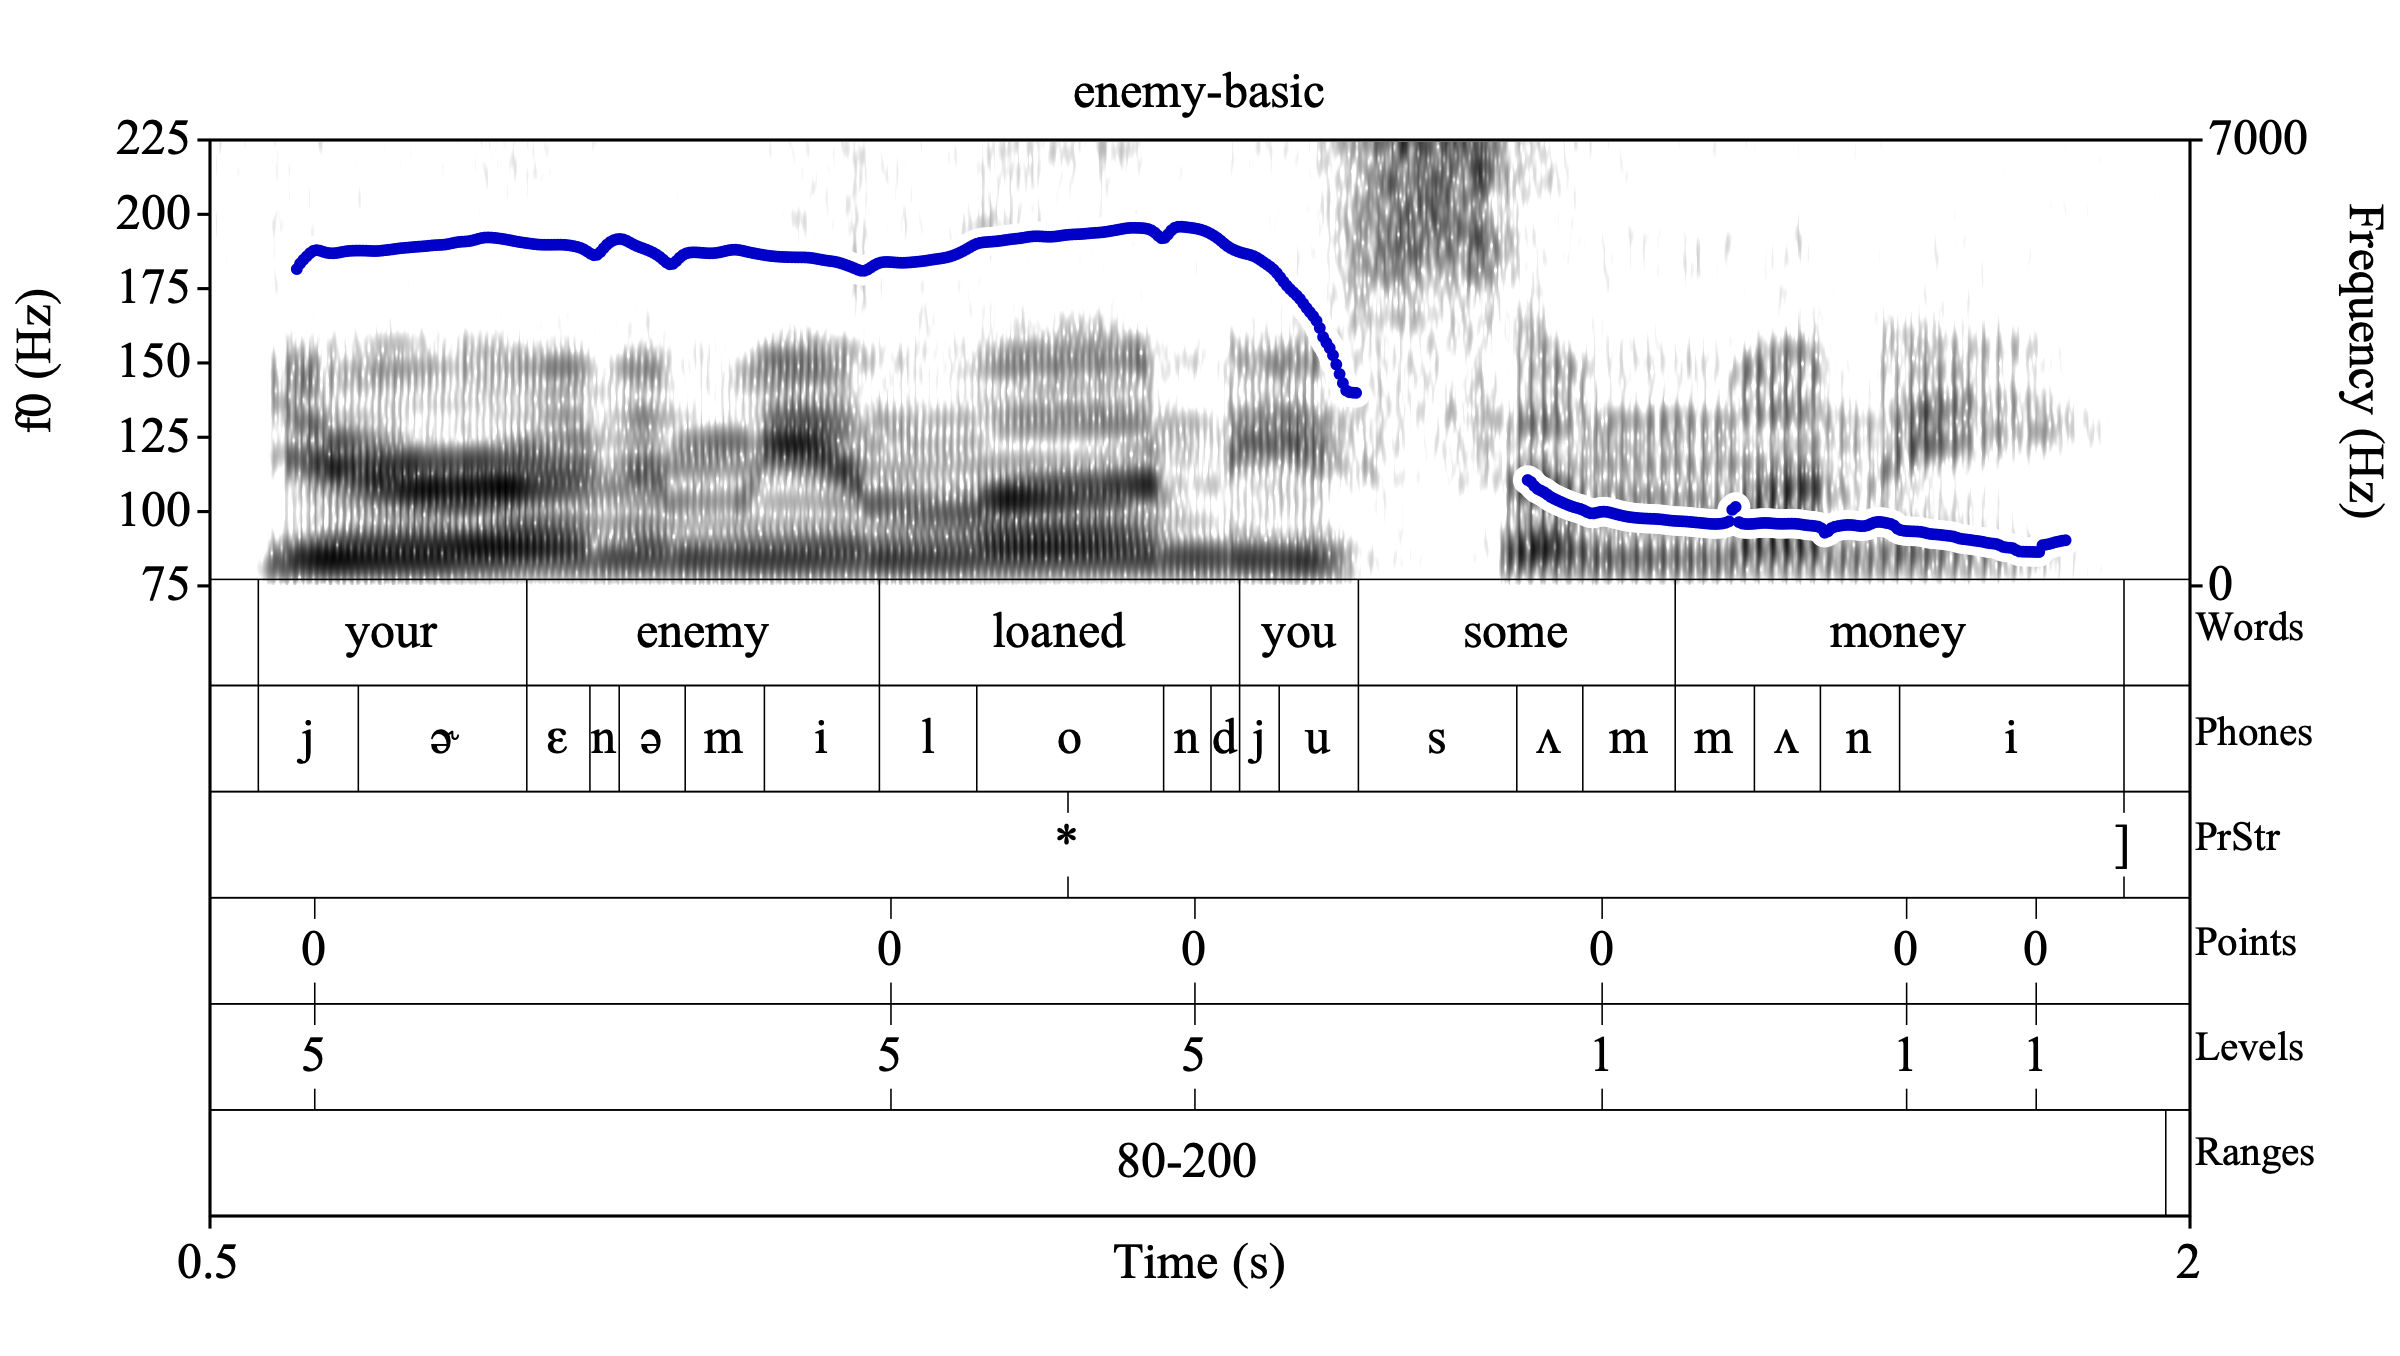
\includegraphics[width=.485\linewidth]{Contours-enemy.png}~~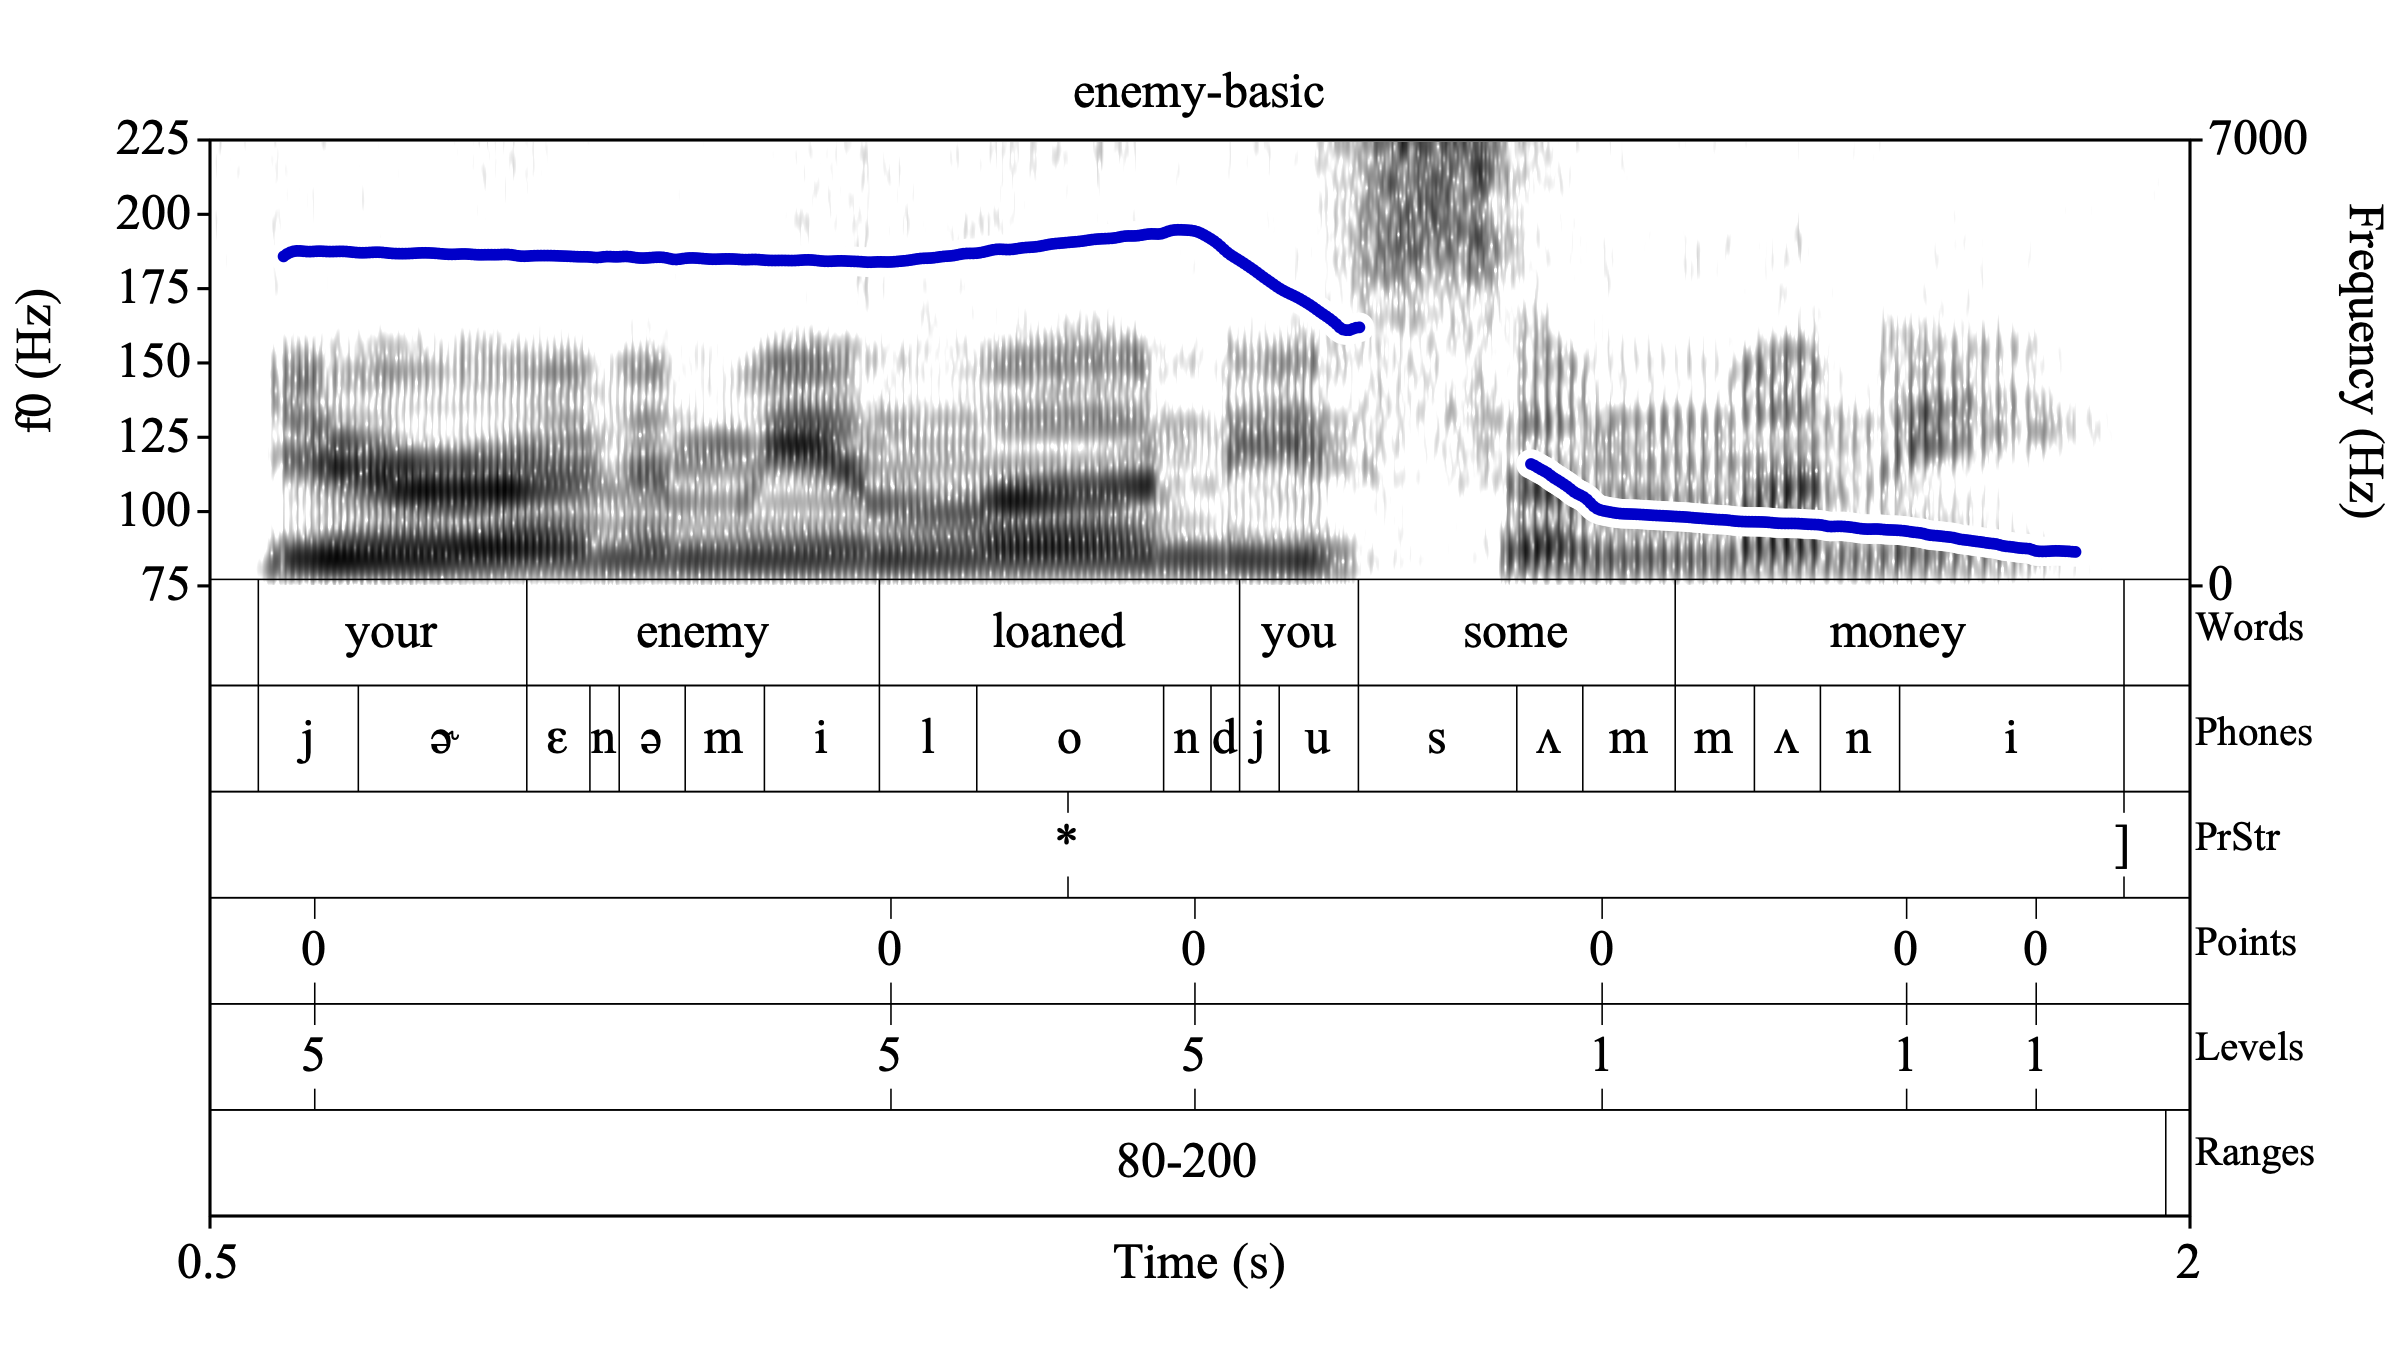
\includegraphics[width=.485\linewidth]{Contours-enemy-resynth.png}
\caption{A recording with PoLaR labels and its resynthesized straight line approximation, created with a script from the PoLaR plugin in Praat.
\label{fig:enemy original and resynth}
}
\end{figure}
Even with such an impoverished version of the pitch track (such as \texttt{enemy-resynth}), and even to a trained ear, the “real” and “resynthesized” examples can be indistinguishable. On the other hand, removing some of these remaining turning points may result in a somewhat “unnatural” sound (in the sense that, at least, a trained ear could distinguish the resynthesized version from the original). Given that this straight line approximation sounds both natural and identical to the original, we argue that our Points tier annotation of six pitch points in Fig. \ref{fig:enemy original and resynth} is sufficient to capture the meaningful turning points. This same technique of manipulating pitch into a straight line approximation can be applied to any recording, to see whether the correct number of Points have been labelled.
Practically speaking, we assume that experienced labellers will be able to distinguish significant turning points from noisy variation, but caution is urged in eliminating those that would impact the shape of the contour. Our experience with the Tonal Center of Gravity dictates that individual Turning points are not perceptually salient; it is the set of turning points that creates a perceptually useful shape. 
In this way, using the Points tier labels to construct a straight-line approximation of the f0 track (which itself is based on the acoustic signal) can be used to help identify the shape of the (abstract phonological) intonational contour.\footnote{Note: this series of acoustic cues in the signal does not, for various reasons (including the phonetics-phonology interface, technical abilities of the pitch tracking software, microprosody, etc.), perfectly reflect the intonational contour, which is an abstract representation (defined in terms of phonological categories and structures).} As such, these straight line approximations have the potential for understanding more about the phonological representation of intonational contours.
\subsection{Sources of f0 track disruptions}\label{sec:a-brief-overview-of-sources-of-pitch-track-disruptions}
As mentioned, while the f0 track is often reflective of the perceptual changes in pitch, there are also regular ways in which the f0 track can differ from the intonational contour. For example, an annotator may perceive the pitch of a portion of the utterance as being steady or moving fluidly, while the f0 track of that region shows a discontinuous f0 contour or one that suddenly jumps up\slash down. Thus, if the labeller over-trusts the visualization in the f0 track (overriding how their auditory pitch perception), this may cause a labeller to label extraneous Points labels to capture movements that are not actually part of the speaker’s intonational contour. (Conversely, the visualization may not seem to show f0 movements even where a labeller auditorily perceives one.) In this section, we discuss some of the more common specific f0 tracking problems that occur, the contexts in which they are likely to arise, and the conventions that have arisen over the years among prosodic labellers for dealing with them.
One class of problems occurs when the software-based f0 estimator is disrupted, leading to breaks in the f0 track. A second kind of problem occurs when contextual factors in the speech\slash recording context distort or influence the f0 track, even though a listener’s perception of the pitch contour is not disrupted by these events. Both of these scenarios can challenge the labeller by complicating the issue of determining where Points labels should(n’t) be added.
When in doubt, the annotator is encouraged to \emph{trust their perception}, because the human mind is especially well-tuned to compensate for these disruptions (producing the abstract and “smoothed” intonation contour, on the basis of intonational competence) while software like Praat is designed to keep track of all f0 movements.
\subsubsection{Software effects}\label{sec:software-effects}
One very common way in which f0 tracks end up as inaccurate (meaning not reflecting listeners’ perception of the pitch) has to do with software settings. Most speech applications (such as Praat) must be calibrated regularly (e.g., re-calibrated for each speaker) to get accurate f0 displays.
An example of settings that can greatly impact f0 tracks is the Pitch range minimum\slash maximum values (in Praat, these are found in Pitch > Pitch settings, in an editor window, when viewing Sound objects). What these settings do is tell the algorithm what the minimum\slash maximum \emph{possible} f0 values are; that is, the algorithm will not entertain the possibility that the f0 values dip below the minimum or above the maximum. As such, if the minimum is set too high (e.g., the minimum is set to 100Hz but the actual f0 gets as low as 75Hz), the software will often produce an f0 track with plotted values that are too high (e.g., plotting f0 values at 160Hz where they ought to be 80Hz; see also §\ref{sec:pitch-halving-and-doubling}). Annotators are encouraged to tailor the Pitch range values for speakers, noting that deeper voiced people typically stay within a range of around 60-300Hz, and higher voiced people typically stay within a range of around 100-500Hz, but this can vary quite a bit from person-to-person (and even from recording to recording).
In addition, Praat (\citealt{praat}) provides various other pitch-related settings, for which we provide values we have found to be helpful in doing intonational analysis of human speech; these are the settings used to produce the figures of f0 tracks in this monograph. (The menus referenced below are found in an editor window).
\begin{itemize}
\item Settings for Time Step analysis (found in \texttt{View> Time step settings}\ldots):
	\begin{itemize}
		\item Time step strategy = fixed
		\item Fixed time step (s) = 0.0025
	\end{itemize} 
\item Advanced Pitch settings (found in \texttt{Pitch> Advanced pitch settings}\ldots):
	\begin{itemize}
		\item Max. number of candidates=15
		\item Very accurate=true
		\item Silence threshold=0.03
		\item Voicing threshold=0.5
		\item Octave cost=0.05
		\item Octave jump cost=0.5
		\item Voiced/Unvoiced cost=0.2
	\end{itemize}
\item[] (\textit{You may find it beneficial to adjust these settings further, in particular recordings, to minimize spurious\slash inaccurate f0 measurements. However, doing so may result in f0 tracks that look different from the ones in this monograph.})
\end{itemize}
Changing these settings may affect the f0 track – for example, changing the voicing threshold and octave jump costs can lead to f0 dropout or spurious f0 readings. This should be taken to reinforce the fact that f0 tracks are meant only as a guide to annotators, and annotators are encouraged to diverge from it when their auditory perception suggests. 
While adjusting software settings (especially Pitch Range minimum\slash maximum) is a way to counteract f0 track disruptions, some f0 disruptions cannot be amended to yield an accurate f0 track, due to insurmountable interference from environmental\slash recording factors (e.g., background noise). In these cases, as described in section \ref{sec:optional-f0-override-labels-for-annotating-pitch-points-without-a-reliable-f0-track}, labellers are encouraged to use their intuition and perception to note an f0 estimate, if appropriate and possible. 
\subsubsection{Pitch halving and doubling}\label{sec:pitch-halving-and-doubling}
Sometimes during a recording, the f0 track will suddenly jump or fall – with the measured f0 jumping from say 199Hz to 97Hz (or vice-versa) from one measured f0 point to the next. When suddenly dropping down by a factor of 2, this is pitch halving. Conversely, when suddenly jumping up by a factor of 2, this is pitch doubling. (The factor of 2 difference is due to how Praat measures f0. Because these jumps are related to the f0 measuring algorithm, they are not always exactly a factor of 2; however, factor-of-2 jumps\slash drops are especially common.) 
In other words, pitch halving and pitch doubling involve a change in measured f0 is immediate and significant – faster than the vocal folds can typically change. An example of pitch halving is given in Figure \ref{fig:to volunteer-halved f0-tracking}, and an example of pitch doubling is given in Figure \ref{fig:rutabaga f0-tracking}.
\begin{figure}[H]
\centering
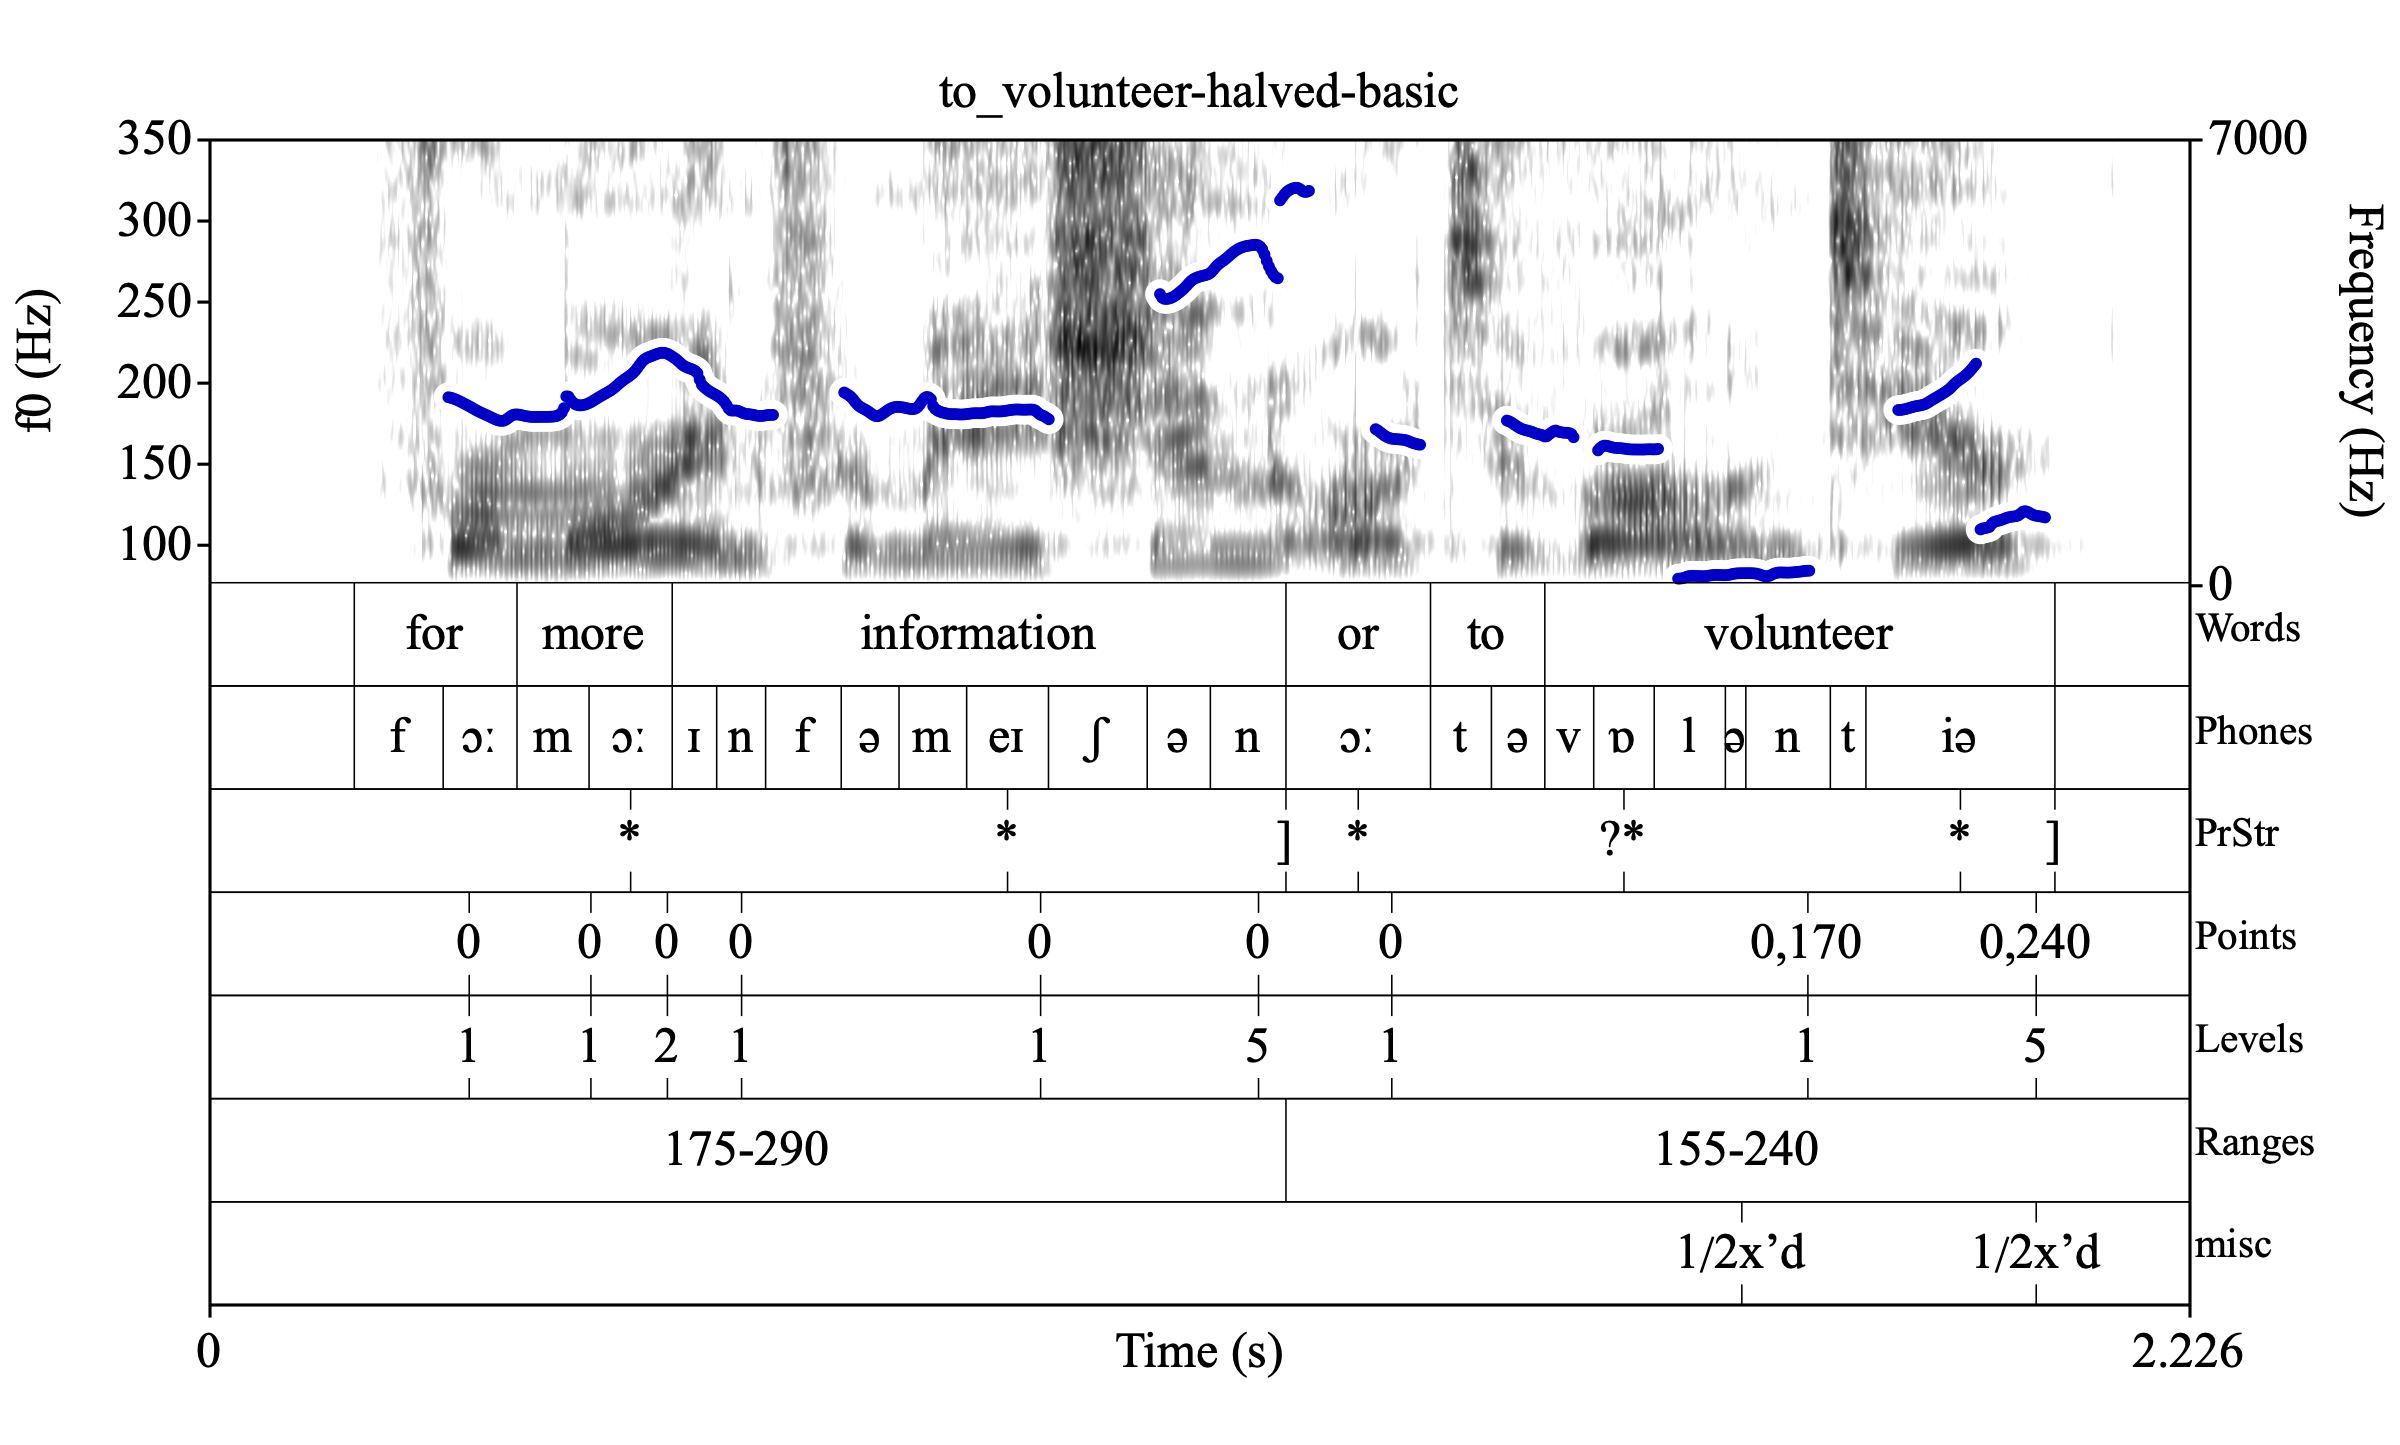
\includegraphics[width=.875\linewidth]{Appendix-to_volunteer-halved.png}
\caption{Example of pitch halving.
\label{fig:to volunteer-halved f0-tracking}
\index{Annotated example, f0 tracking!to\_volunteer-halved}
}
\end{figure}
\begin{figure}[H]
\centering
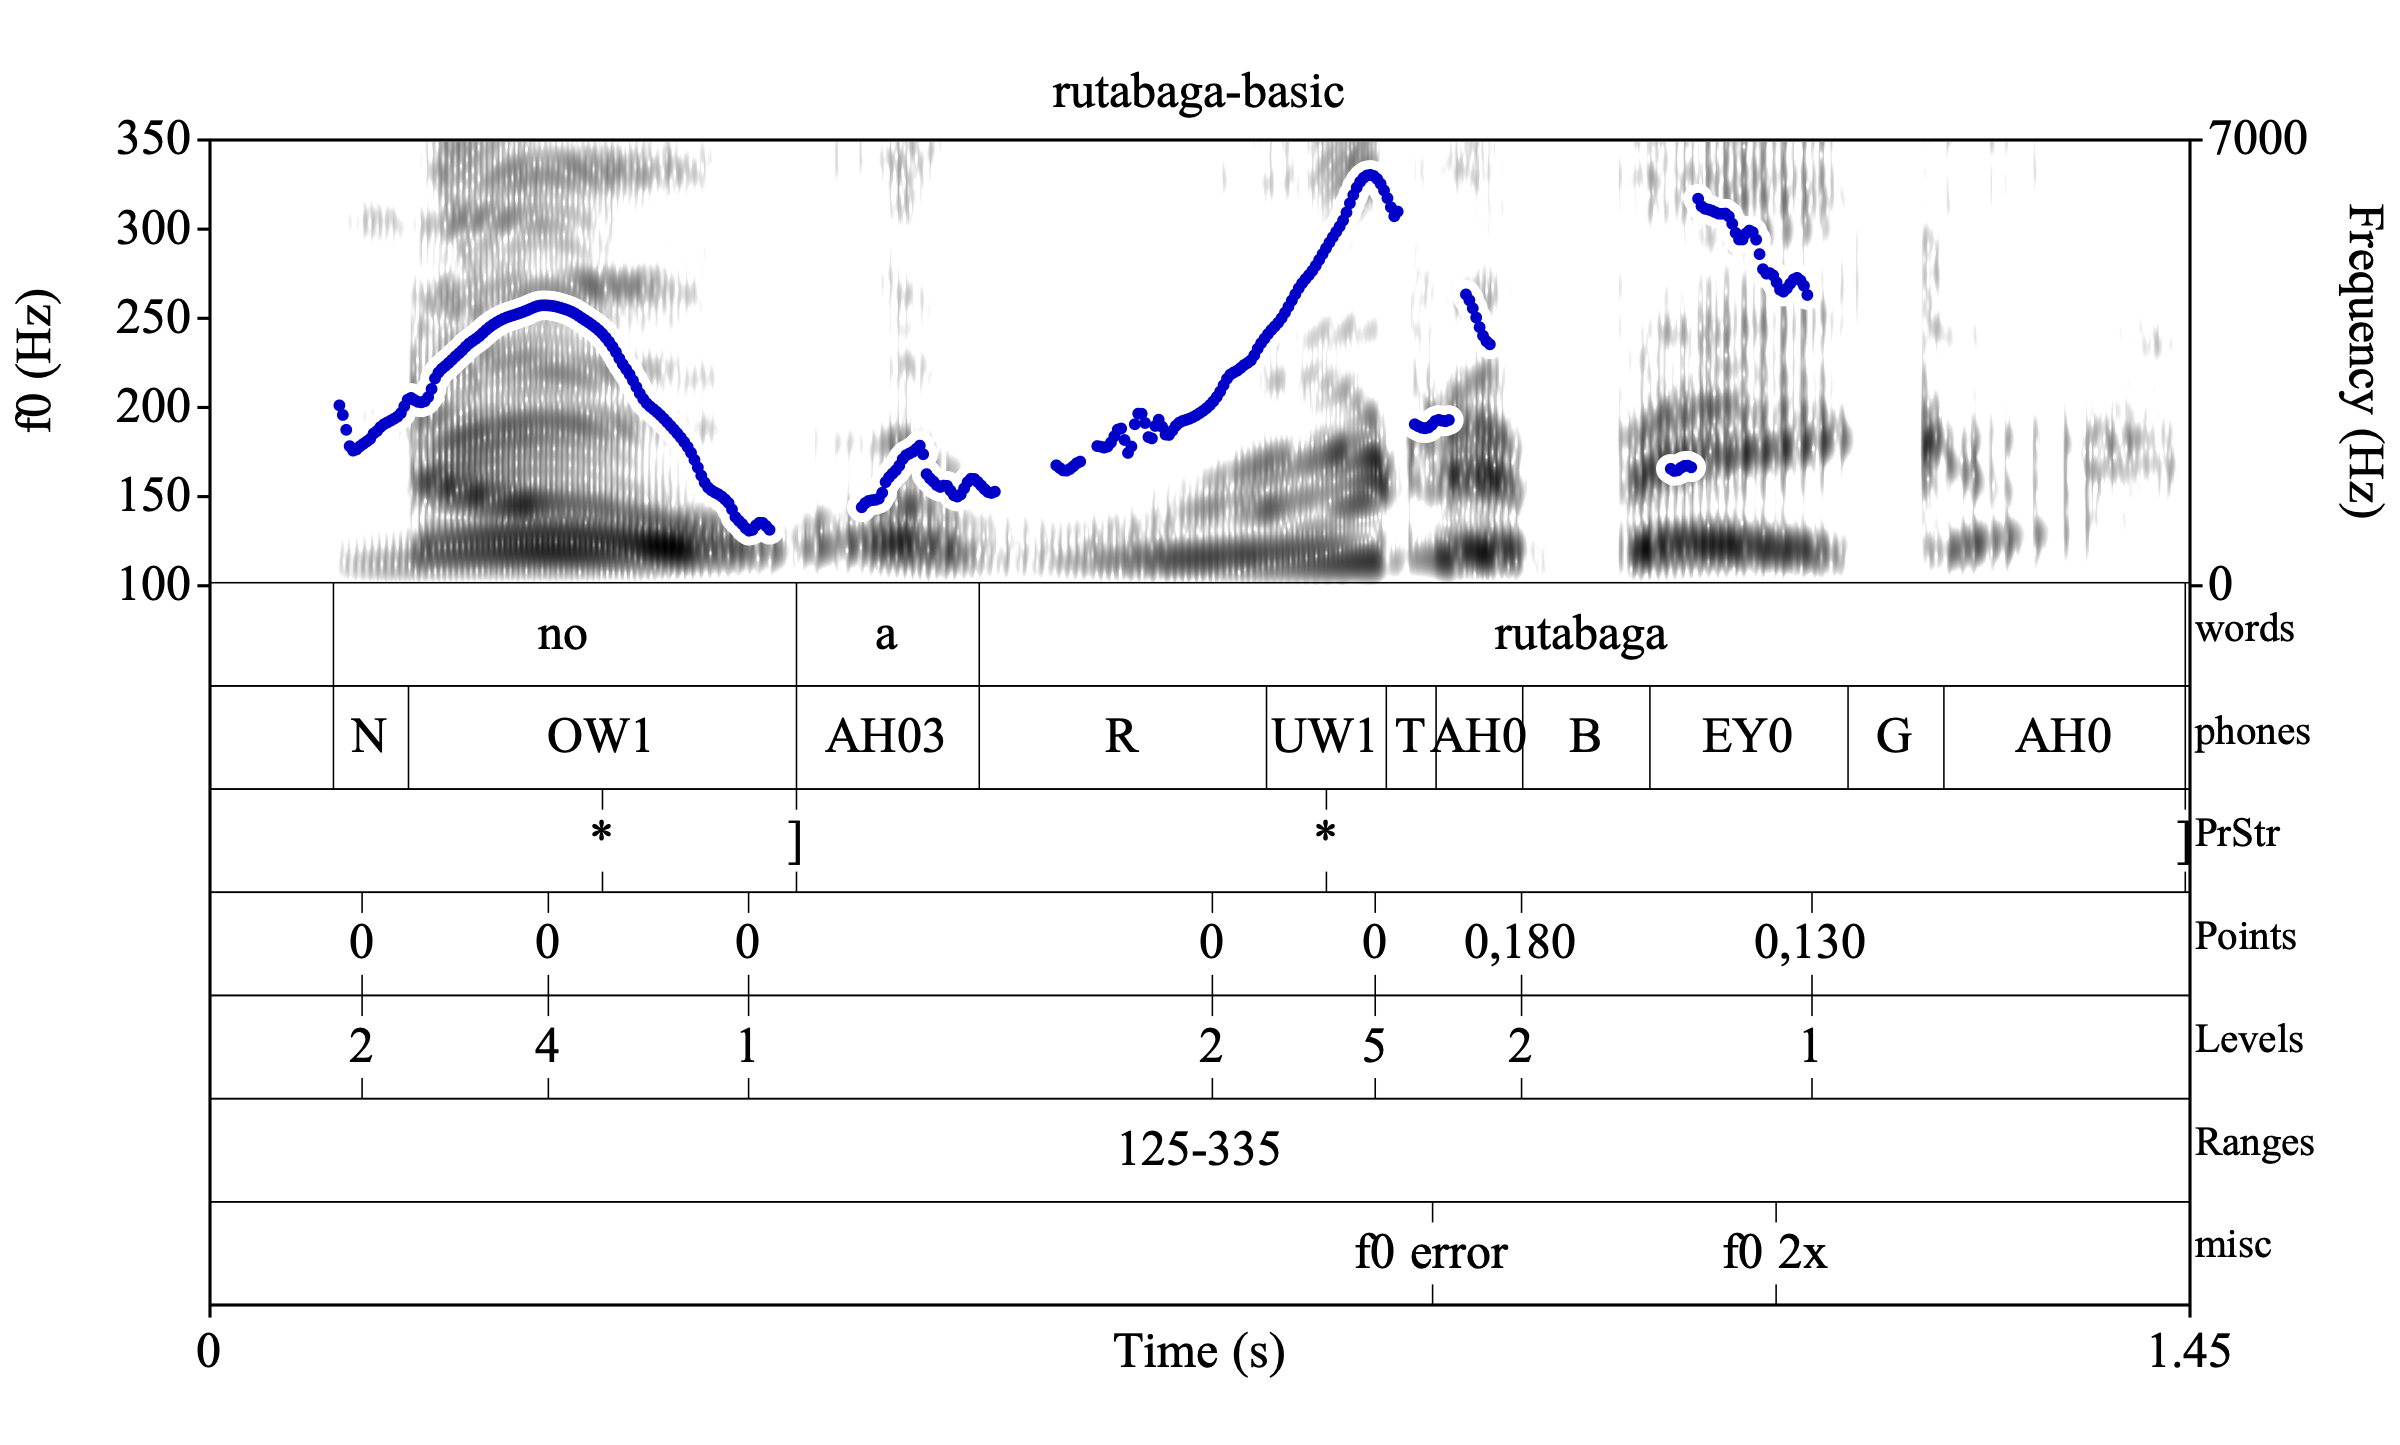
\includegraphics[width=.875\linewidth]{Contours-rutabaga-basic.png}
\caption{Example of pitch doubling.
\label{fig:rutabaga f0-tracking}
\index{Annotated example, f0 tracking!rutabaga}
}
\end{figure}
We provide some hints to help identify what is “immediate and significant”, a labeller can rely on.
First and foremost, a labeller should trust their auditory perception. If the labeller perceives that the pitch is locally low, but the f0 track looks locally high, this could be due to pitch doubling; for example, at the end of “\langtext{rutabaga}” in Fig. \ref{fig:to volunteer-halved f0-tracking}, the pitch is perceived to continually fall, but it shows as almost as high as the preceding peak. Similarly, if the f0 shows a low that sounds high to the labeller, this may be halving. In these cases, the f0 tracker commonly measures f0 values that are either half (e.g., the pitch tracker shows 70 Hz, where listeners perceive pitch corresponding to 140 Hz) or double (e.g., the pitch tracker shows 140 Hz, where listeners perceive pitch corresponding to 70 Hz) the “true” pitch for the speech.
A second way is to try changing the pitch range settings. If the pitch range settings are set to 100-200Hz, but the true f0 max is 250Hz, any f0 that is truly between 200Hz and 250Hz will be mis-measured – often as pitch halving, showing as 100-125Hz. This is because, if a speaker reaches a peak f0 over 500Hz but your maximum is set at 400Hz, the f0 tracker will be forced to estimate points within that range. Adjusting the setting for the pitch range maximum to be 250Hz will often resolve this sort of pitch halving. However, there are cases of pitch halving\slash doubling that persist even when the pitch range is set appropriately (such as Fig. \ref{fig:rutabaga f0-tracking}).
The third way we name here to check perception is to make use of the tool for resynthesizing straight line approximations (as described in section \ref{sec:identifying-necessary-points-labels-with-straight-line-approximations}). In Fig. \ref{fig:to volunteer-halved f0-tracking}, there are no Points labels during the pitch-halved regions, and resynthesizing yields a recording that sounds like the original. Had the drop in measured f0 been faithful to a drop in the true f0, such a resynthesis without Points labels encoding the drops would sound like a different contour. For Fig. \ref{fig:rutabaga f0-tracking}, a comma override is used; at the time of the final Points label, the f0 tracker reads about 260Hz, so a comma override of \textlabel{,130} (i.e., half the measured value) is used. The resynthesis of Fig. \ref{fig:rutabaga f0-tracking} is shown in Fig. \ref{fig:rutabaga-resynth f0-tracking}, below, and it sounds very much like the original.
\begin{figure}[H]
\centering
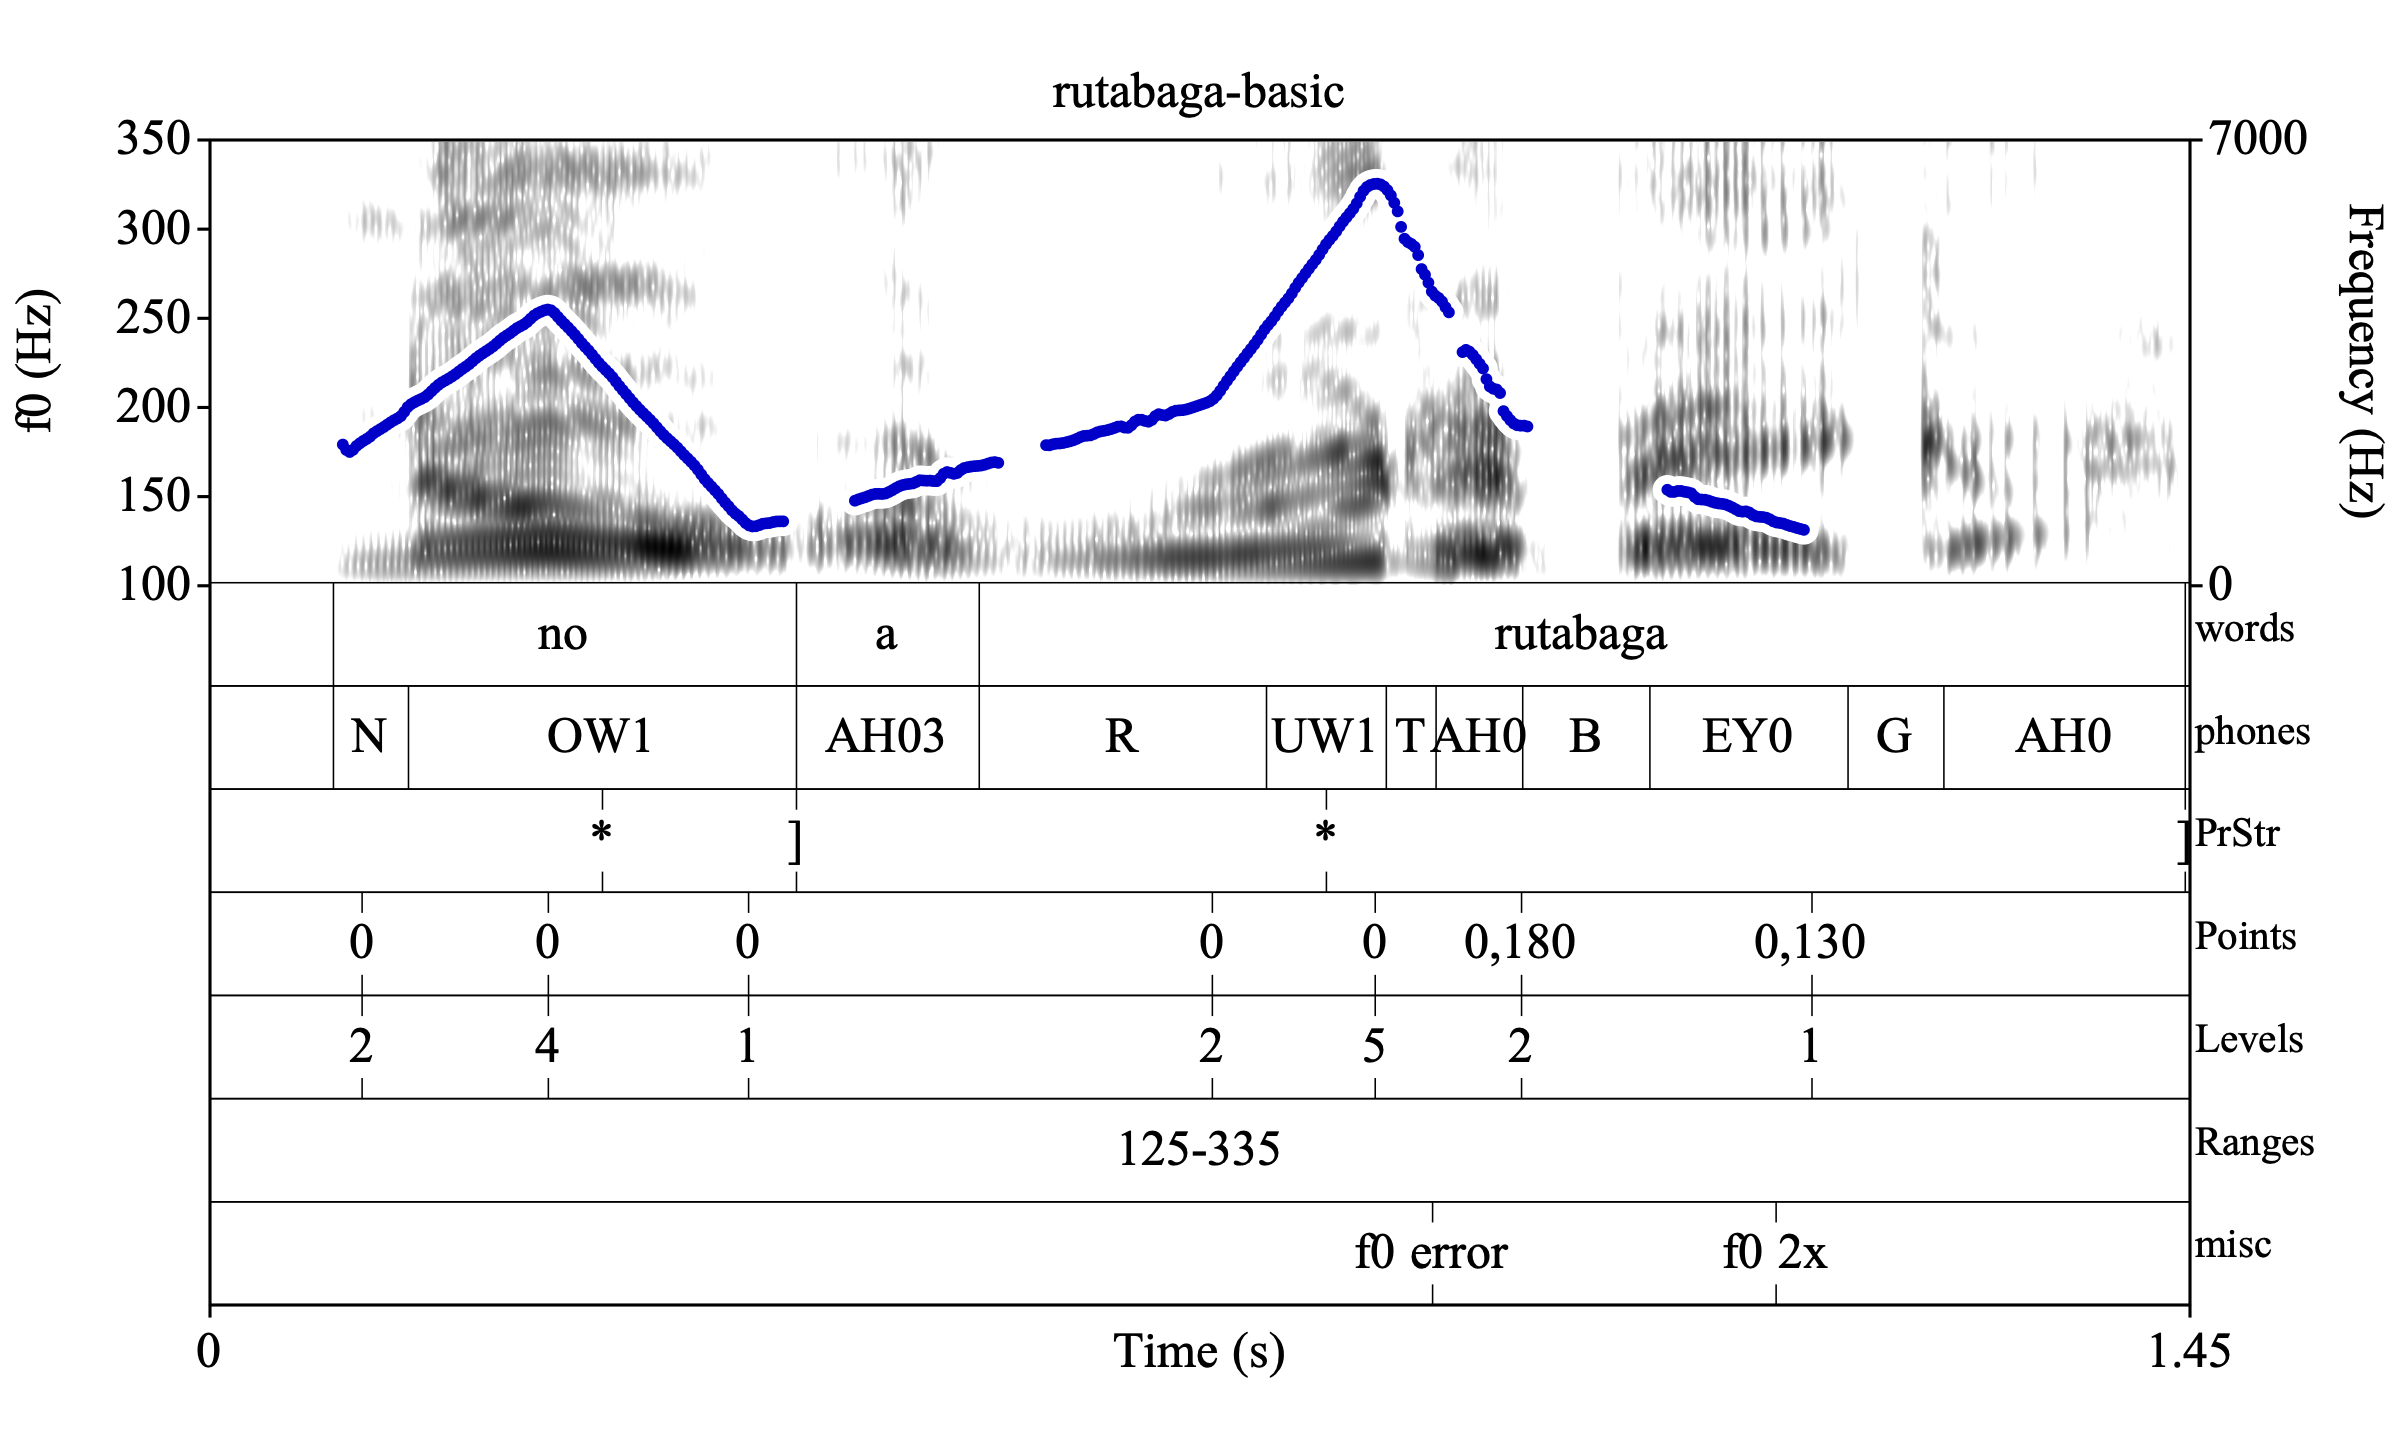
\includegraphics[width=.875\linewidth]{Contours-rutabaga-basic-resynth.png}
\caption{A resynthesis that is perceptually equivalent to the original that exhibited pitch doubling.
\label{fig:rutabaga-resynth f0-tracking}
\index{Annotated example, f0 tracking!rutabaga}
}
\end{figure}
In the coming sections, we discuss some common sources of f0 tracking disruptions, that are due to the speech signal itself (and not the software or its settings).
\subsubsection{Segmental effects}\label{sec:segmental-effects}
Another very common set of cases where adjusting software settings may do enough to yield a clean f0 track have to do with the nature of the phonetic characteristics of certain speech sounds. (As noted earlier, these segmental effects are also known as “microprosodic” effects.) Because f0 tracks rely on regular and identifiable repeating patterns in the speech signal, and because speech sounds vary with respect to these properties, the f0 track is frequently influenced by the segments themselves. Some of the core types of segmental effects on f0 tracks are listed here:
\begin{itemize}
\item Voiceless segments: i.e., segments during which there is at least an interval where there is no vocal fold vibration. These are the most straightforward interruptions of the pitch track.
\item Distortions of f0 in the vicinity of obstruents (stops and fricatives): bumps up or down in f0 at the transitions between a consonant and a neighboring segment, or during a voiced fricative
\item Intrinsic pitch of certain vowels: [i] has a higher intrinsic pitch, [a] has a lower one 
\item[] (\uline{HINT}: Sonorant sounds yield fewer segmental effects on pitch, because they involve the most regular and most easily identifiable acoustic patterns with respect to f0.)
\end{itemize}
Consider the example in figure \ref{fig:marmalade cake f0-tracking}, which has the same intonational contour overlaid on utterances with very different segments. The first portion of the recording, “\langtext{Mariana made the marmalade}”, is mostly smooth and steady, because it is primarily composed of sonorant sounds (except the [d] and [ð], where the pitch track is notably less reliable). On the other hand, the second portion of the recording, “\langtext{Jack baked the cake}”, is much less reliable: during the stops and affricates in this utterance, Praat is unable to detect f0. Thus this is an example where the intonational contours are essentially the same, while the f0 tracks are very different, due to segmental effects.
\begin{figure}[H]
\centering
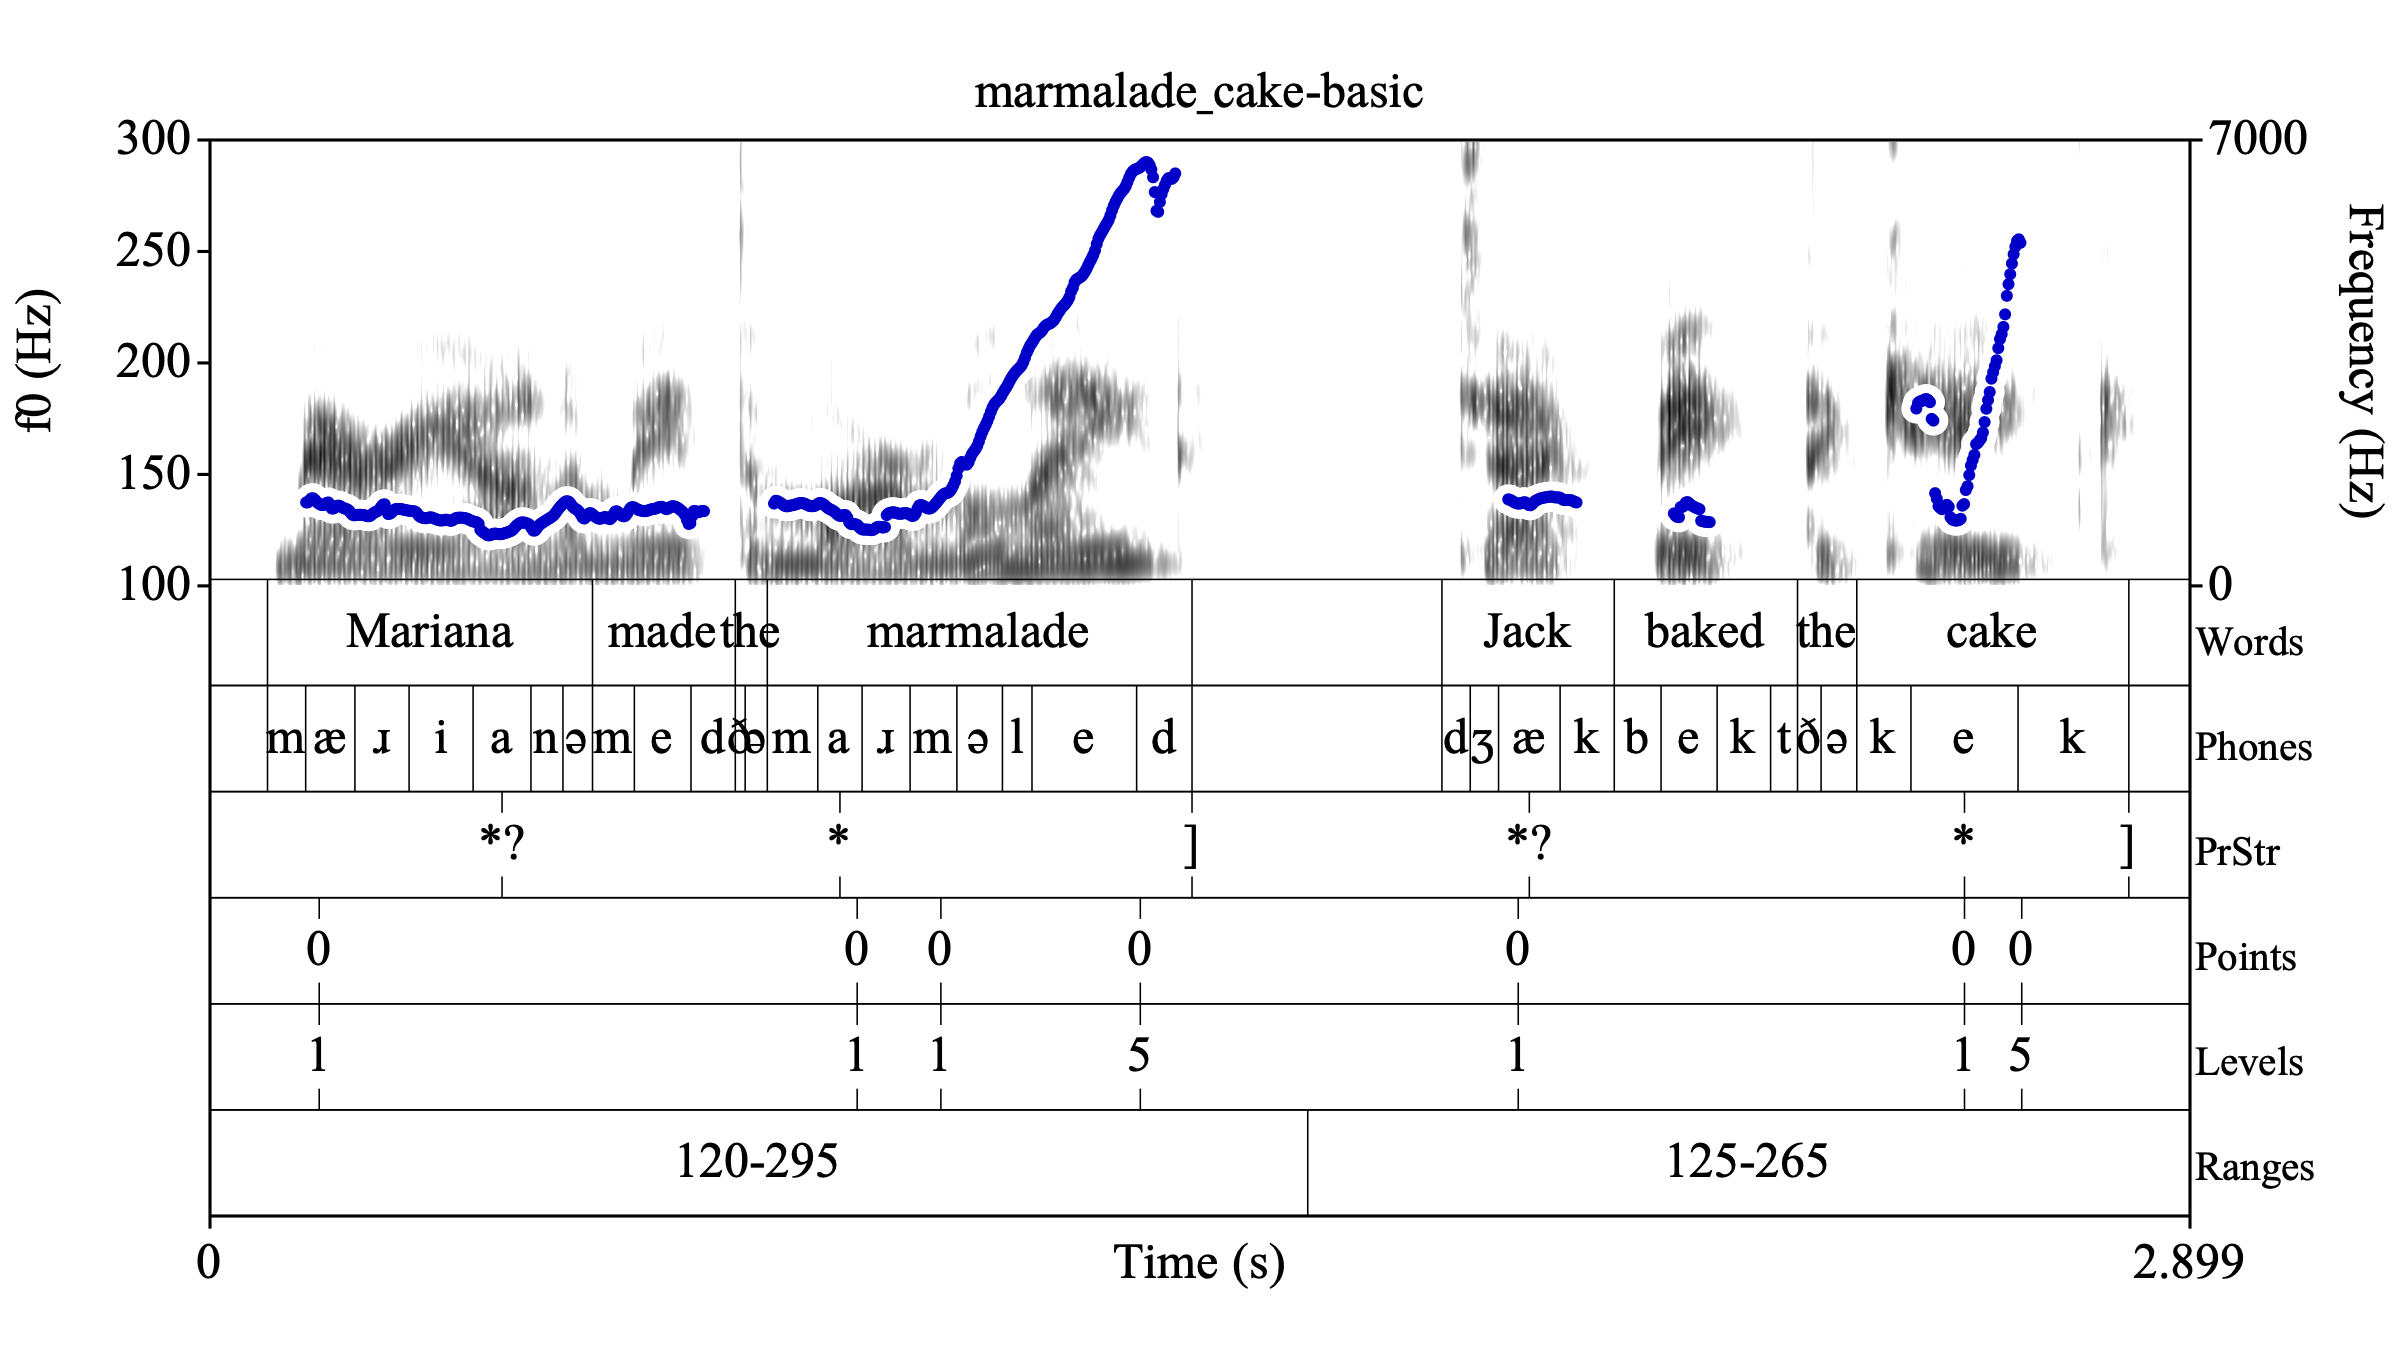
\includegraphics[width=.875\linewidth]{Appendix-marmalade_cake.png}
\caption{The same intonational melody applied to a sentence largely comprised of sonorant sounds (left) and to a sentence with many non-sonorants (right).
\label{fig:marmalade cake f0-tracking}
\index{Annotated example, f0 tracking!marmalade\_cake}
}
\end{figure}
The example in figure \ref{fig:design improvements f0-tracking} shows additional examples where the f0 track is heavily distorted by non-sonorant sounds.  In particular, note that the [z] in “\langtext{design}” and the [mp] in “\langtext{improvements}” both cause a significant drops in the f0 track, but they do not correspond to drops in pitch – listening to this example, labellers perceive the pitch as rising steadily from the beginning of “\langtext{design}” to the peak in “\langtext{improvements}”, as reflected by the Points tier labels (which skip over the two mentioned drops in f0).
\begin{figure}[H]
\centering
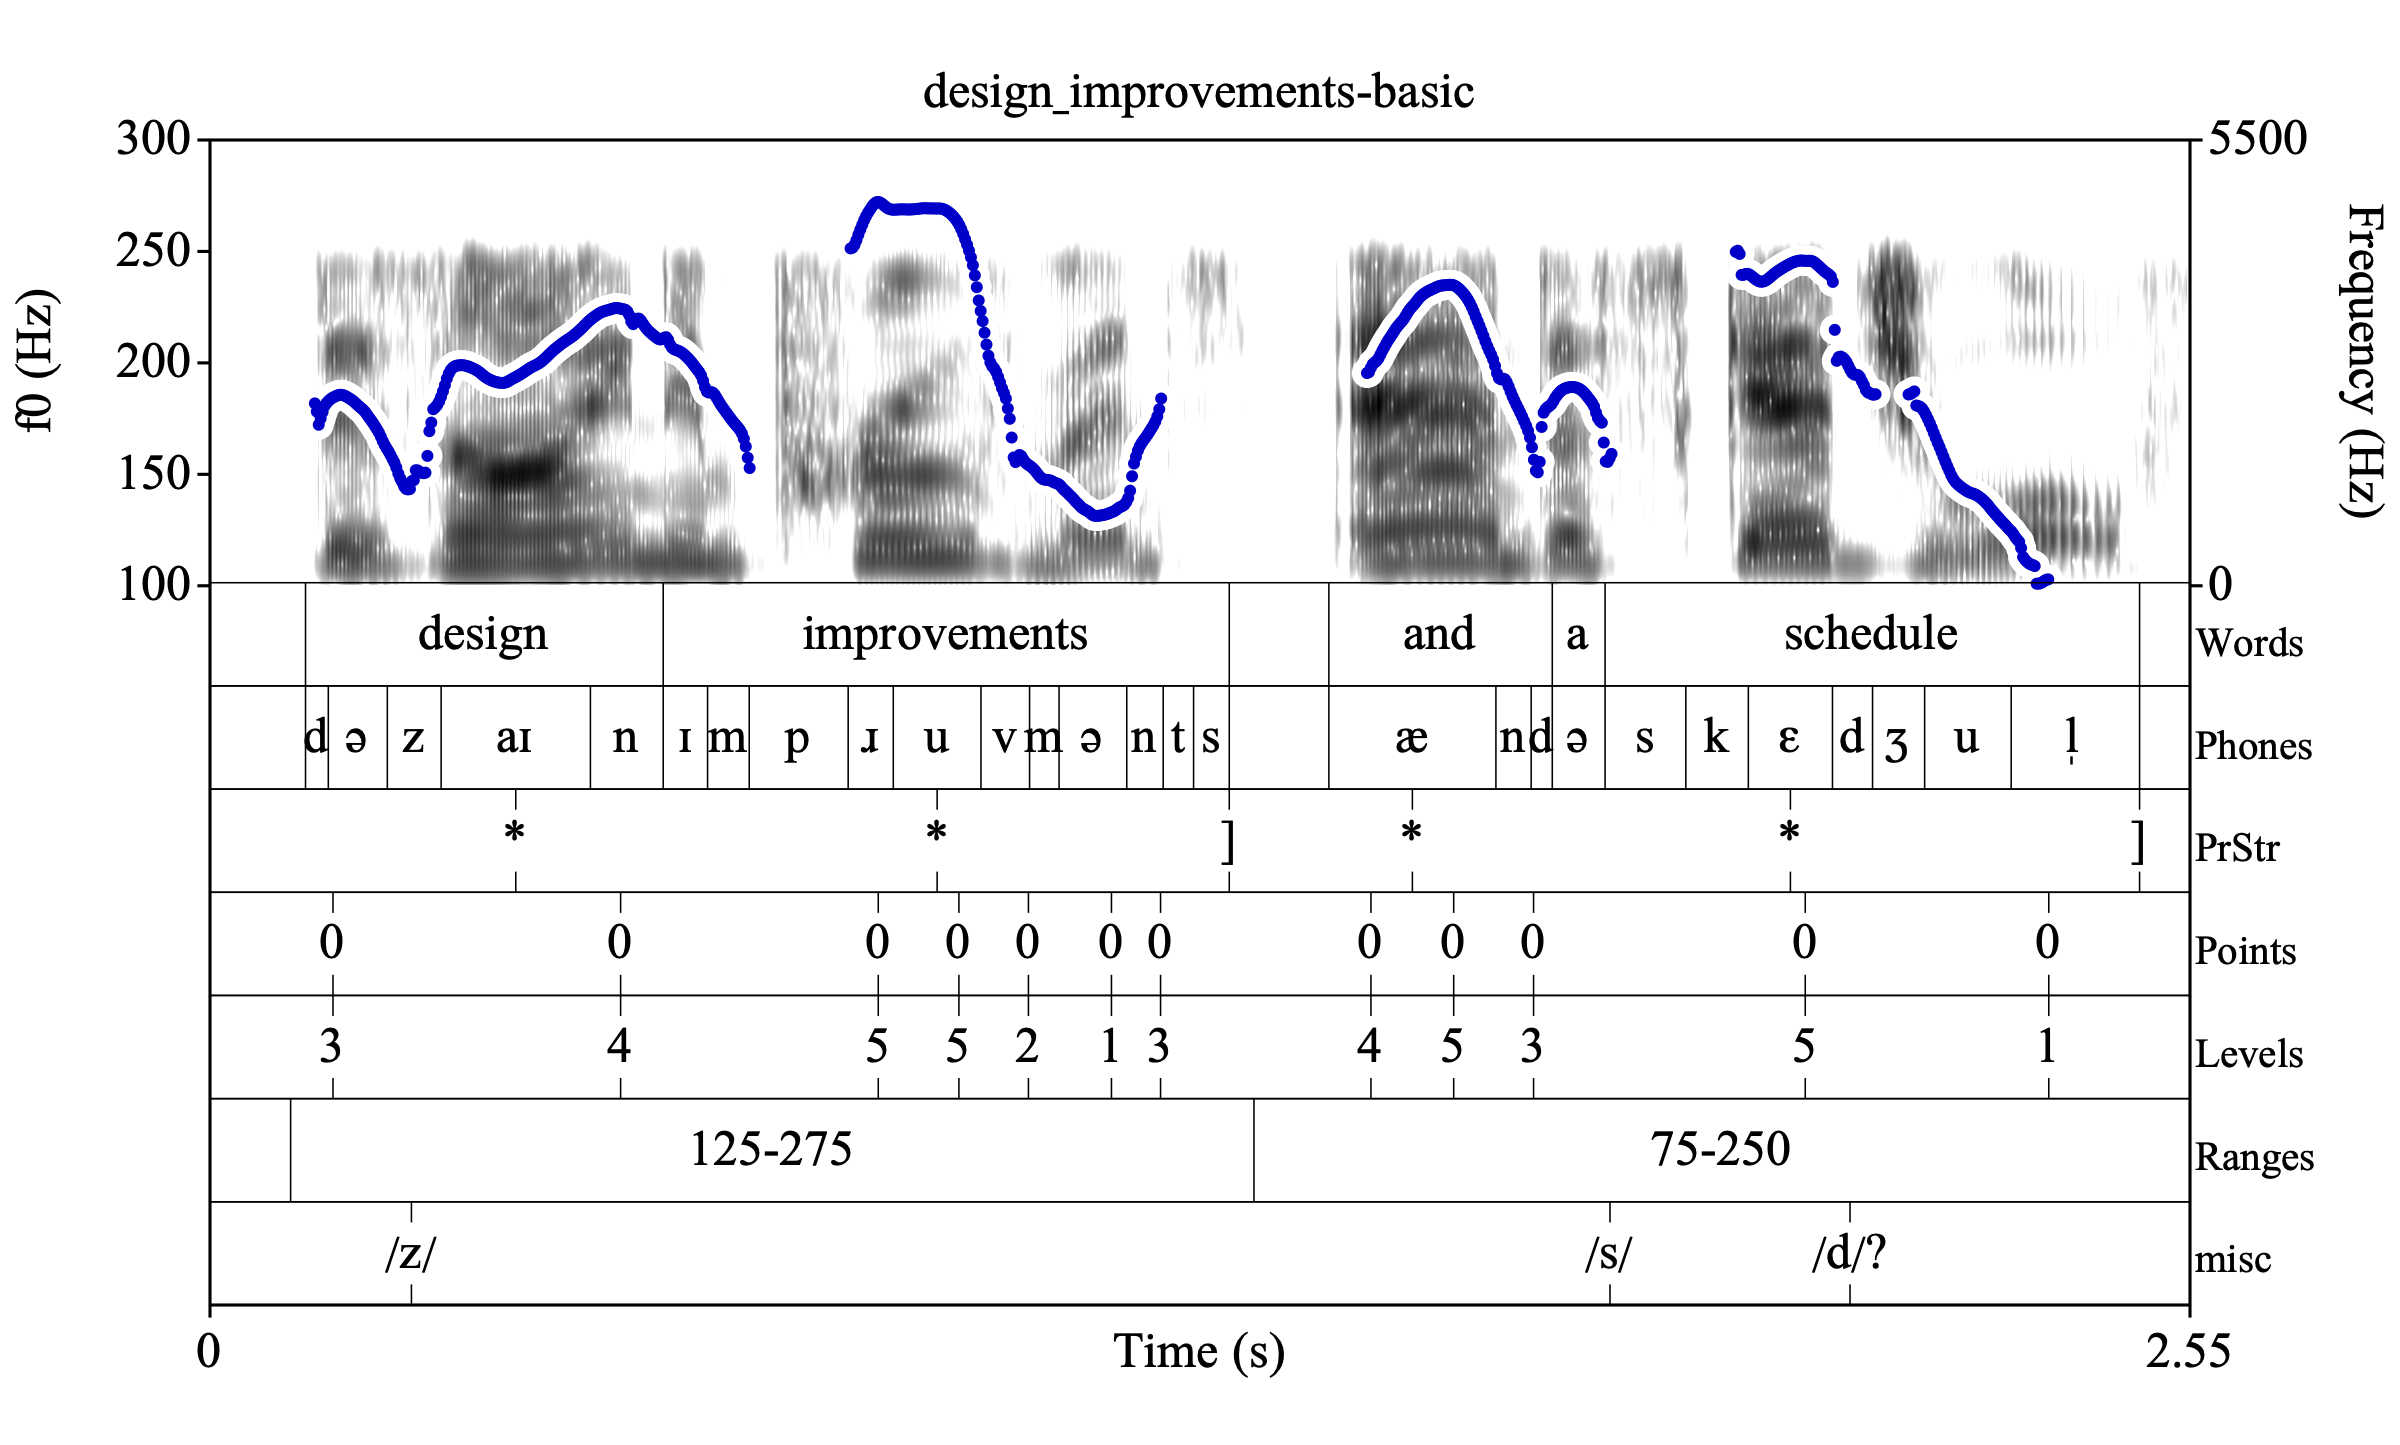
\includegraphics[width=.875\linewidth]{Appendix-design_improvements.png}
\caption{An example where non-sonorant sounds disturb the f0 tracking; this is especially noticeable in the [z] of “\langtext{design}” and [p] of “\langtext{improvements}”.
\label{fig:design improvements f0-tracking}
\index{Annotated example, f0 tracking!design\_improvements}
}
\end{figure}
Consider now the example in figure \ref{fig:out of order-plateau f0-tracking}, which exhibits many small rises\slash falls in the f0 track. Note that the Points tier annotations reflect that the annotators perceive the pitch containing many fewer turning points – for example, the Points annotation reflects a mostly steady pitch during “\langtext{seems like it’s}”. This perception of much smoother pitch is reflected in the straight line approximation resynthesis in figure \ref{fig:out of order-plateau f0-tracking}.
\begin{figure}[H]
\centering
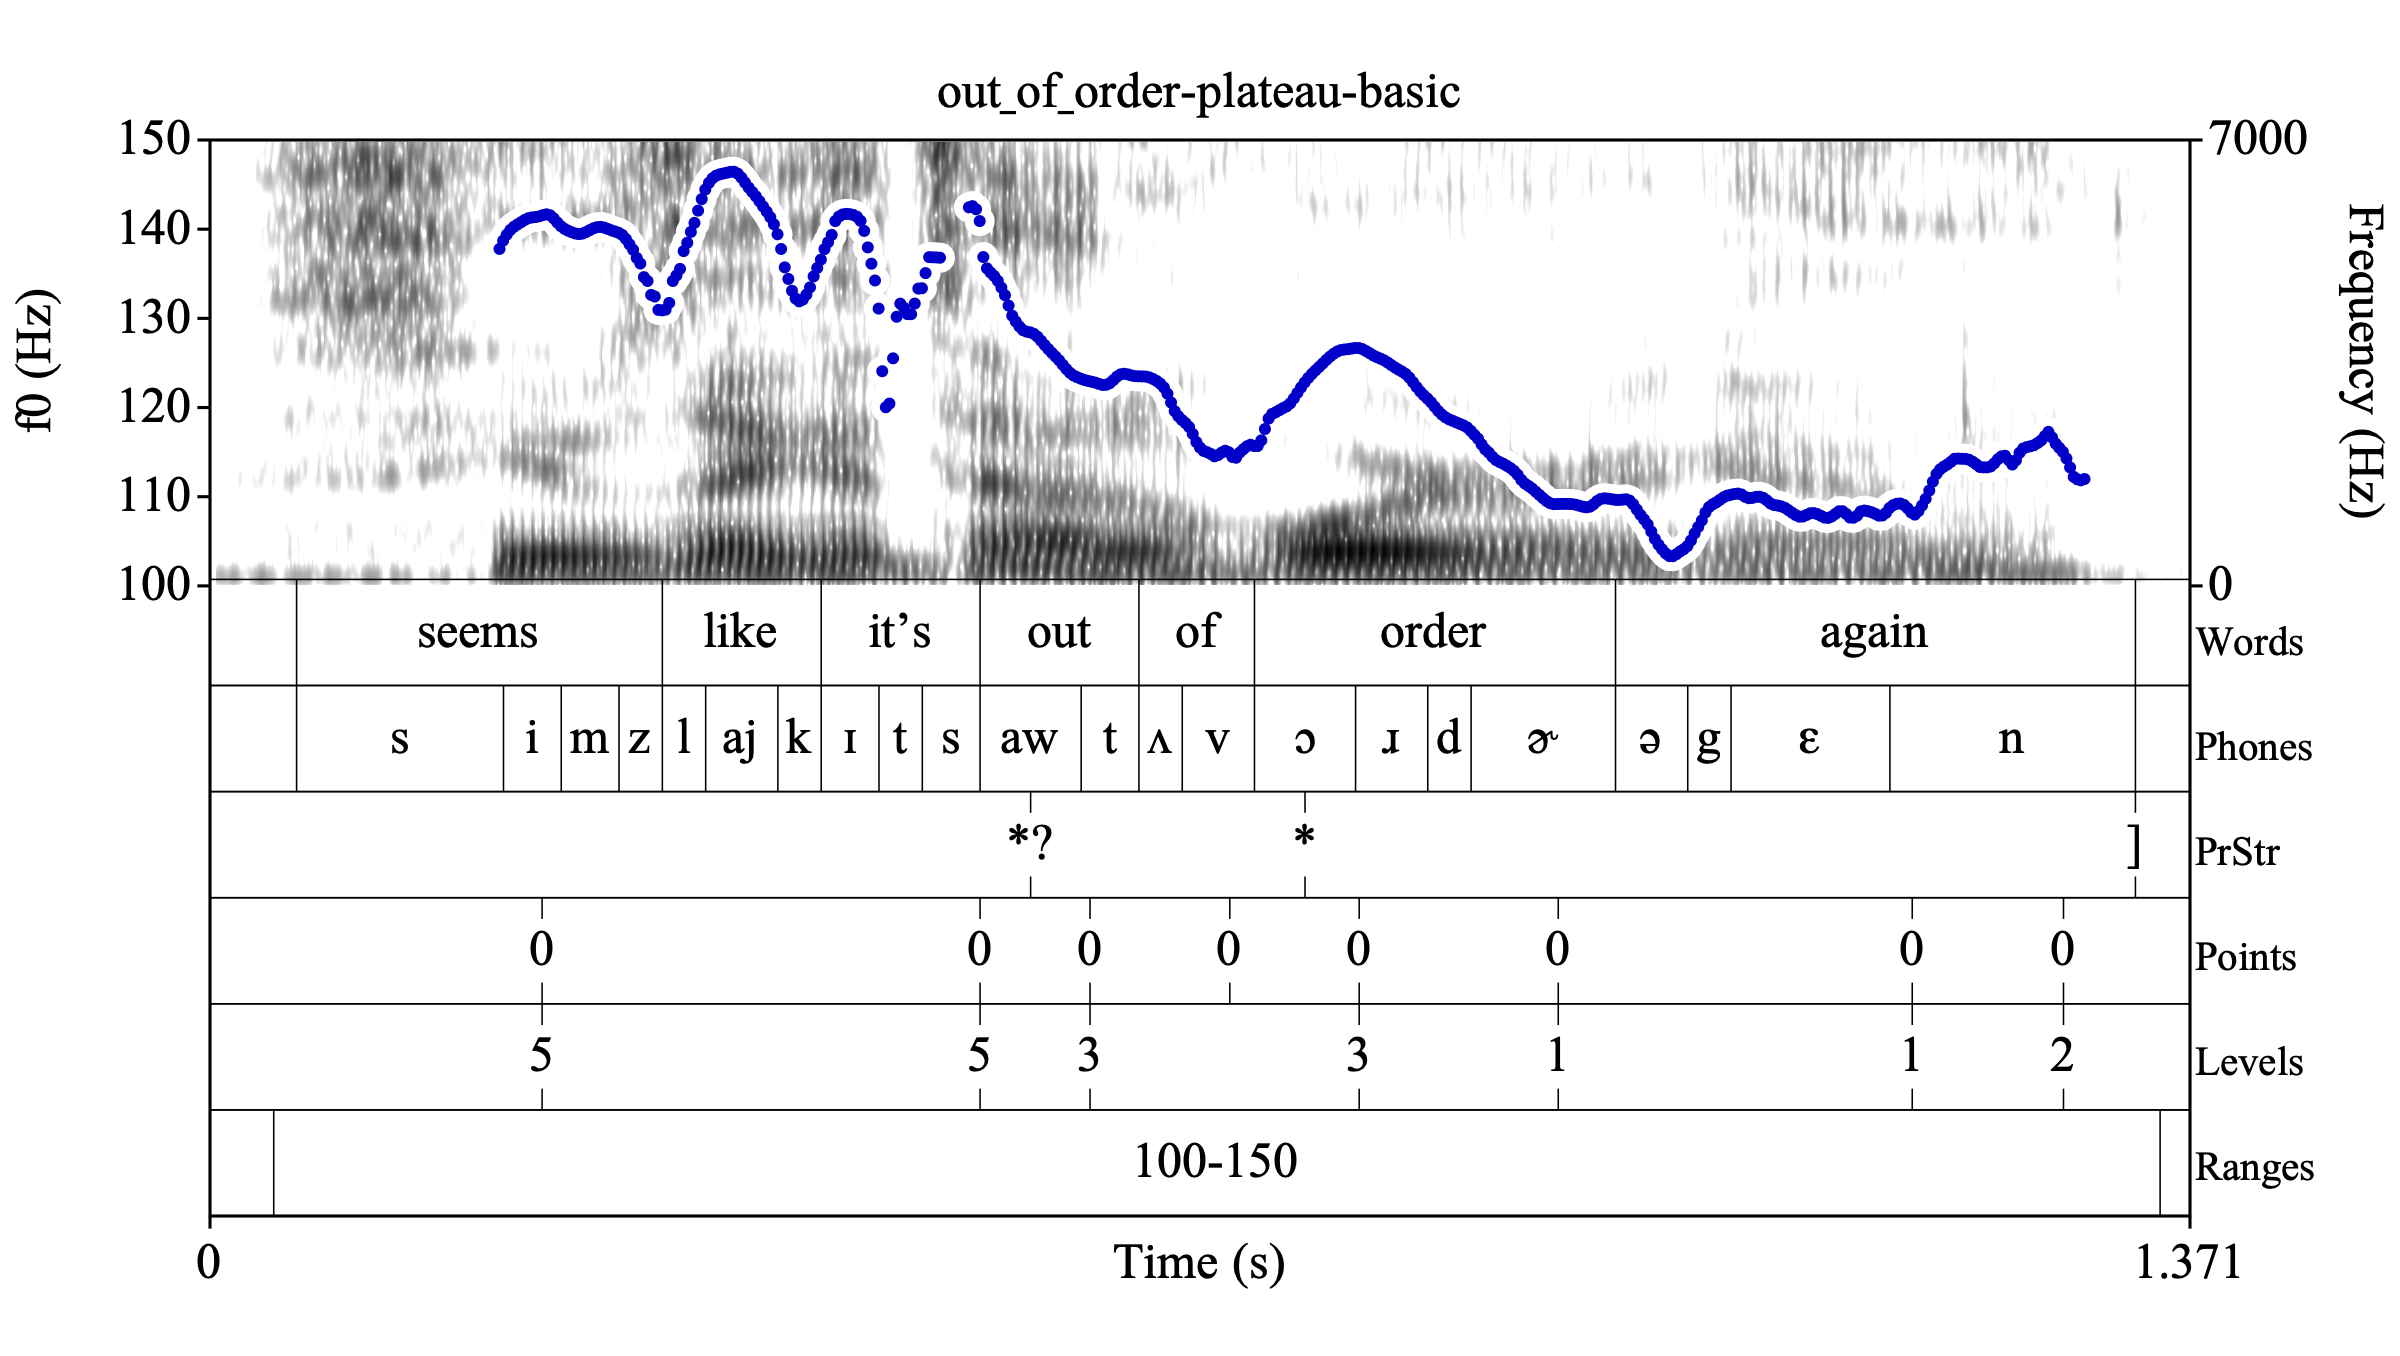
\includegraphics[width=.875\linewidth]{Appendix-out_of_order-plateau}
\caption{An example with lots of perturbations in the f0, due to segmental effects.
\label{fig:out of order-plateau f0-tracking}
\index{Annotated example, f0 tracking!out\_of\_order-plateau}
}
\end{figure}
\begin{figure}[H]
\centering
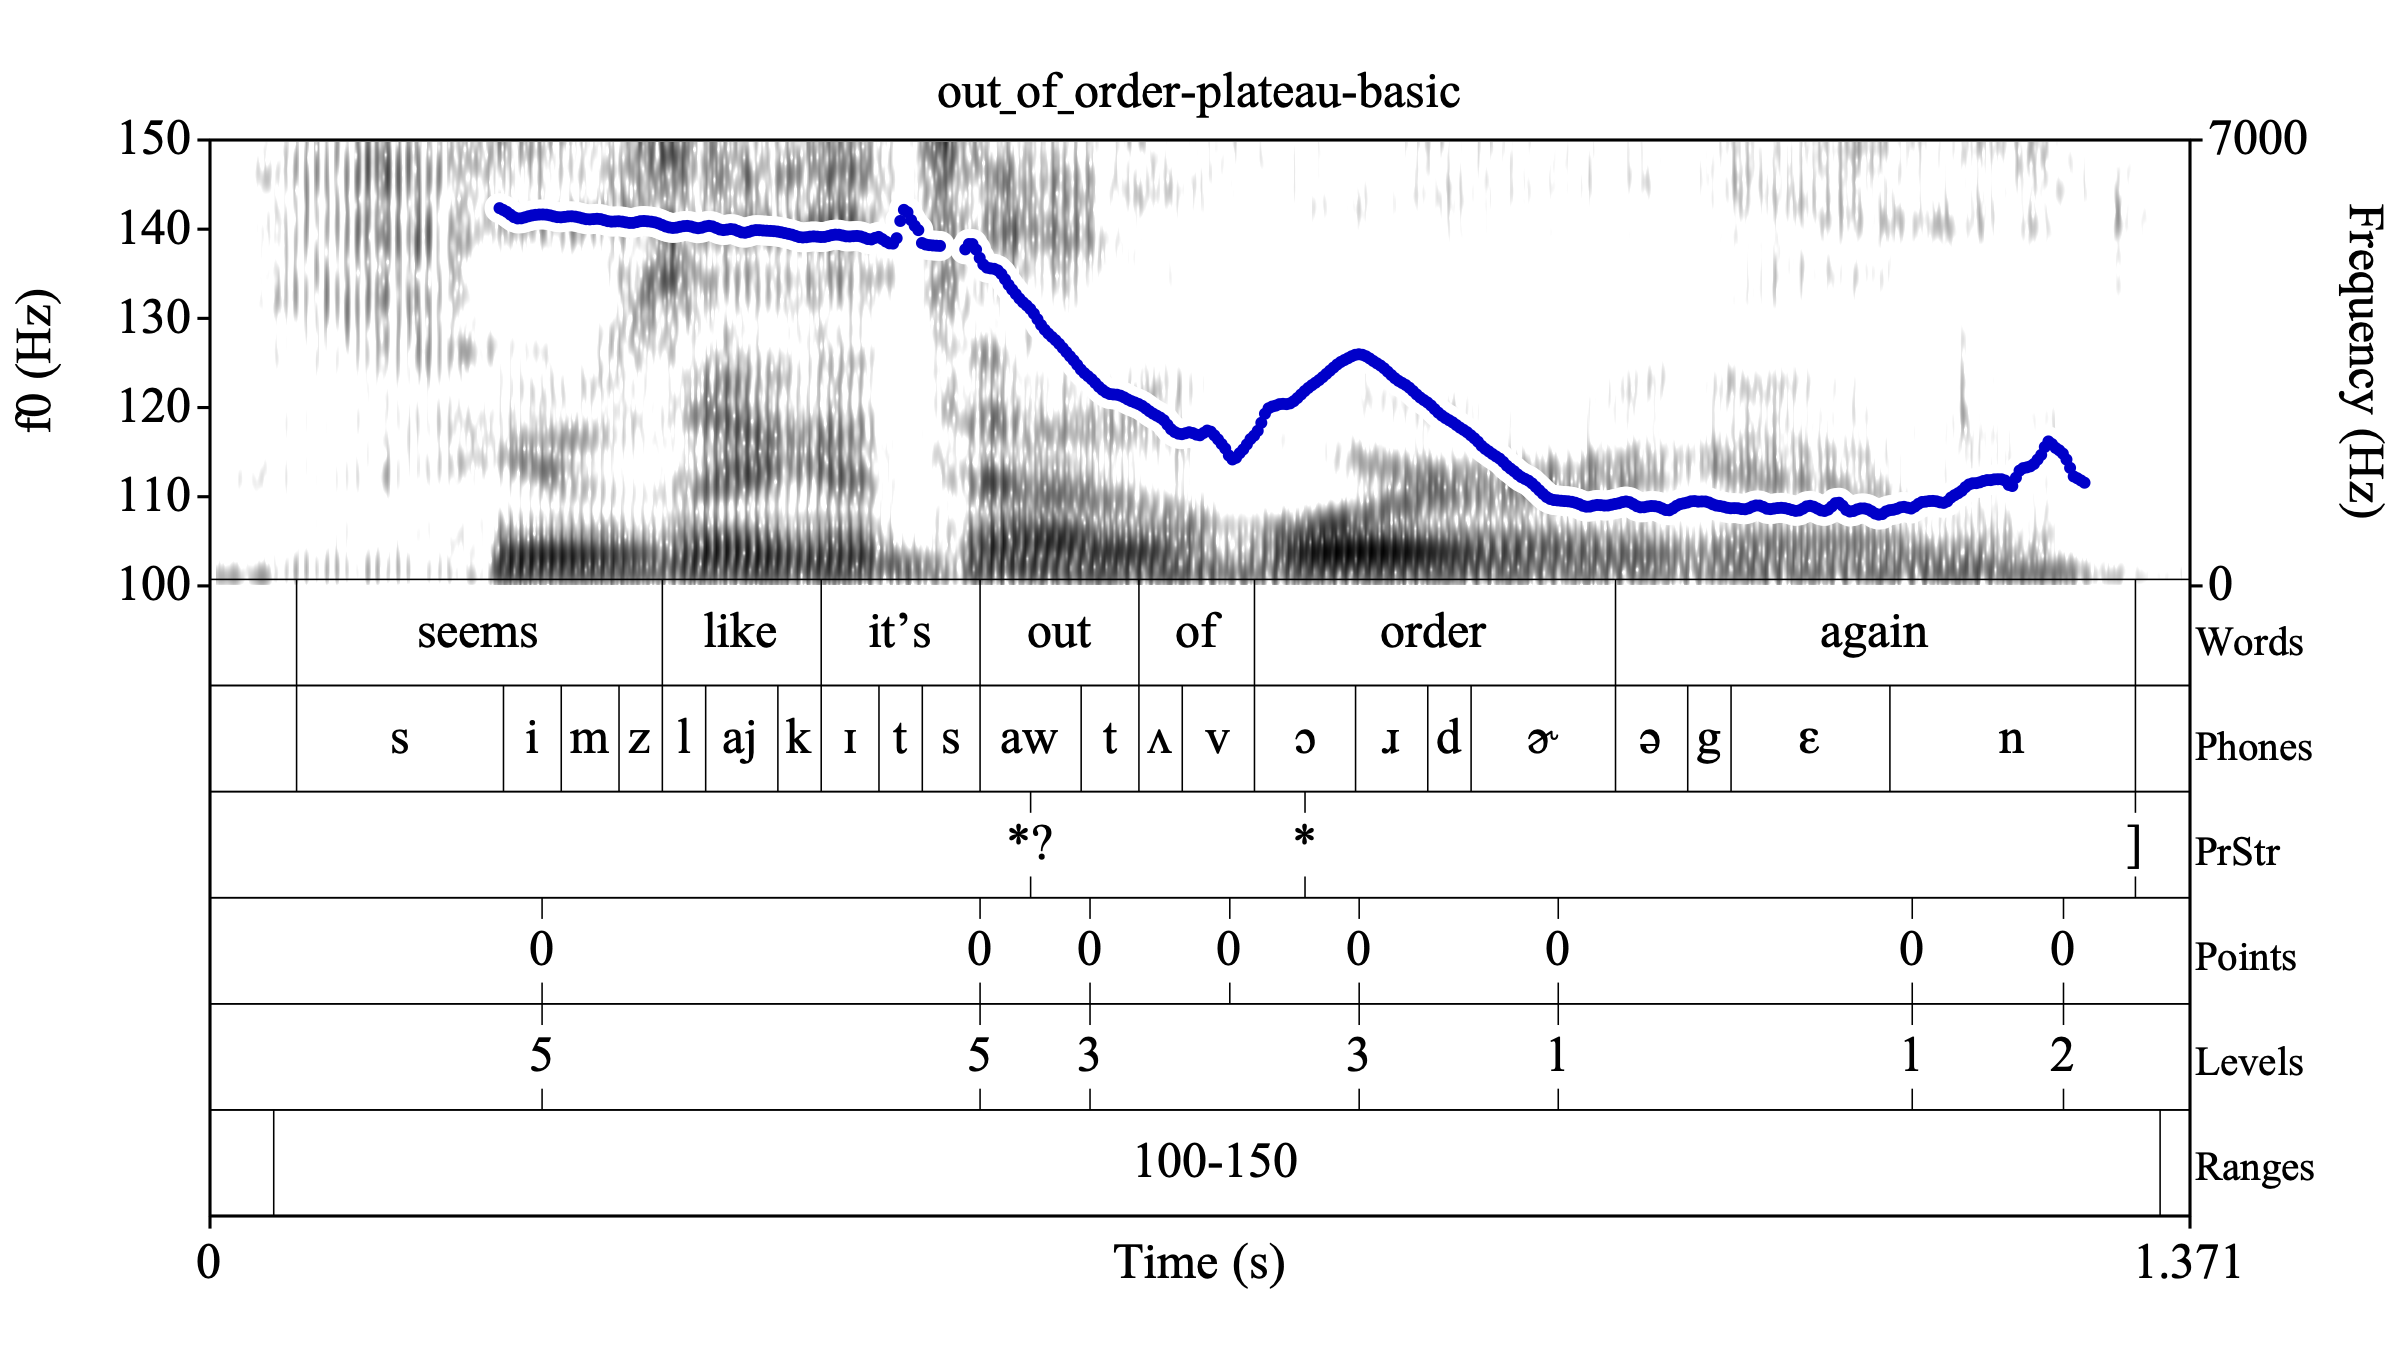
\includegraphics[width=.875\linewidth]{Appendix-out_of_order-plateau-resynth}
\caption{A resynthesis on the basis of the Points annotation, to reflect the much smoother intonational contour that the annotator perceives.
\label{fig:out of order-plateau f0-tracking}
}
\end{figure}
\subsubsection{Voice quality effects}\label{sec:voice-quality-effects}
In addition to speech segments affecting how f0 is tracked, the voice quality of speech can also impact f0 tracking. (\uline{NOTE}: Voice quality effects —especially from creakiness— are especially common at the edges of prosodic groups.) Voice quality (a.k.a. phonation) refers to how the vocal folds (and the larynx more broadly) are configured during speech production. Modal voice (the “neutral” voice quality) does not impact f0 tracking, while other phonations such as creaky voice, breathy voice, and whisper voice can and do regularly impact f0 tracking. For example, during whispering or breathiness, the f0 track may be absent or values may appear somewhat scattered. 
A particularly frequent non-modal phonation is creaky voice; it is especially common at the ends of phrases and where the pitch is low. It is marked by irregular pitch periods and especially perceptual glottalization (which can be seen in a spectrogram as prominent vertical striations, as during the bulk of the final [i] in Fig. \ref{fig:joey f0-tracking}). During creaky voice, the f0 may disappear or appear to jump suddenly upwards\slash downwards. Both of these effects can be seen in Fig. \ref{fig:joey f0-tracking}: there is creaky voice during “\langtext{it to}” and at the end of “\langtext{Joey}”; during “\langtext{it to}” there is no f0 tracking, and during “\langtext{Joey}”, the f0 tracking jumps suddenly upwards (at the beginning of [i]) and then disappears until the speaker returns to modal voice at the end of the utterance.
\begin{figure}[H]
\centering
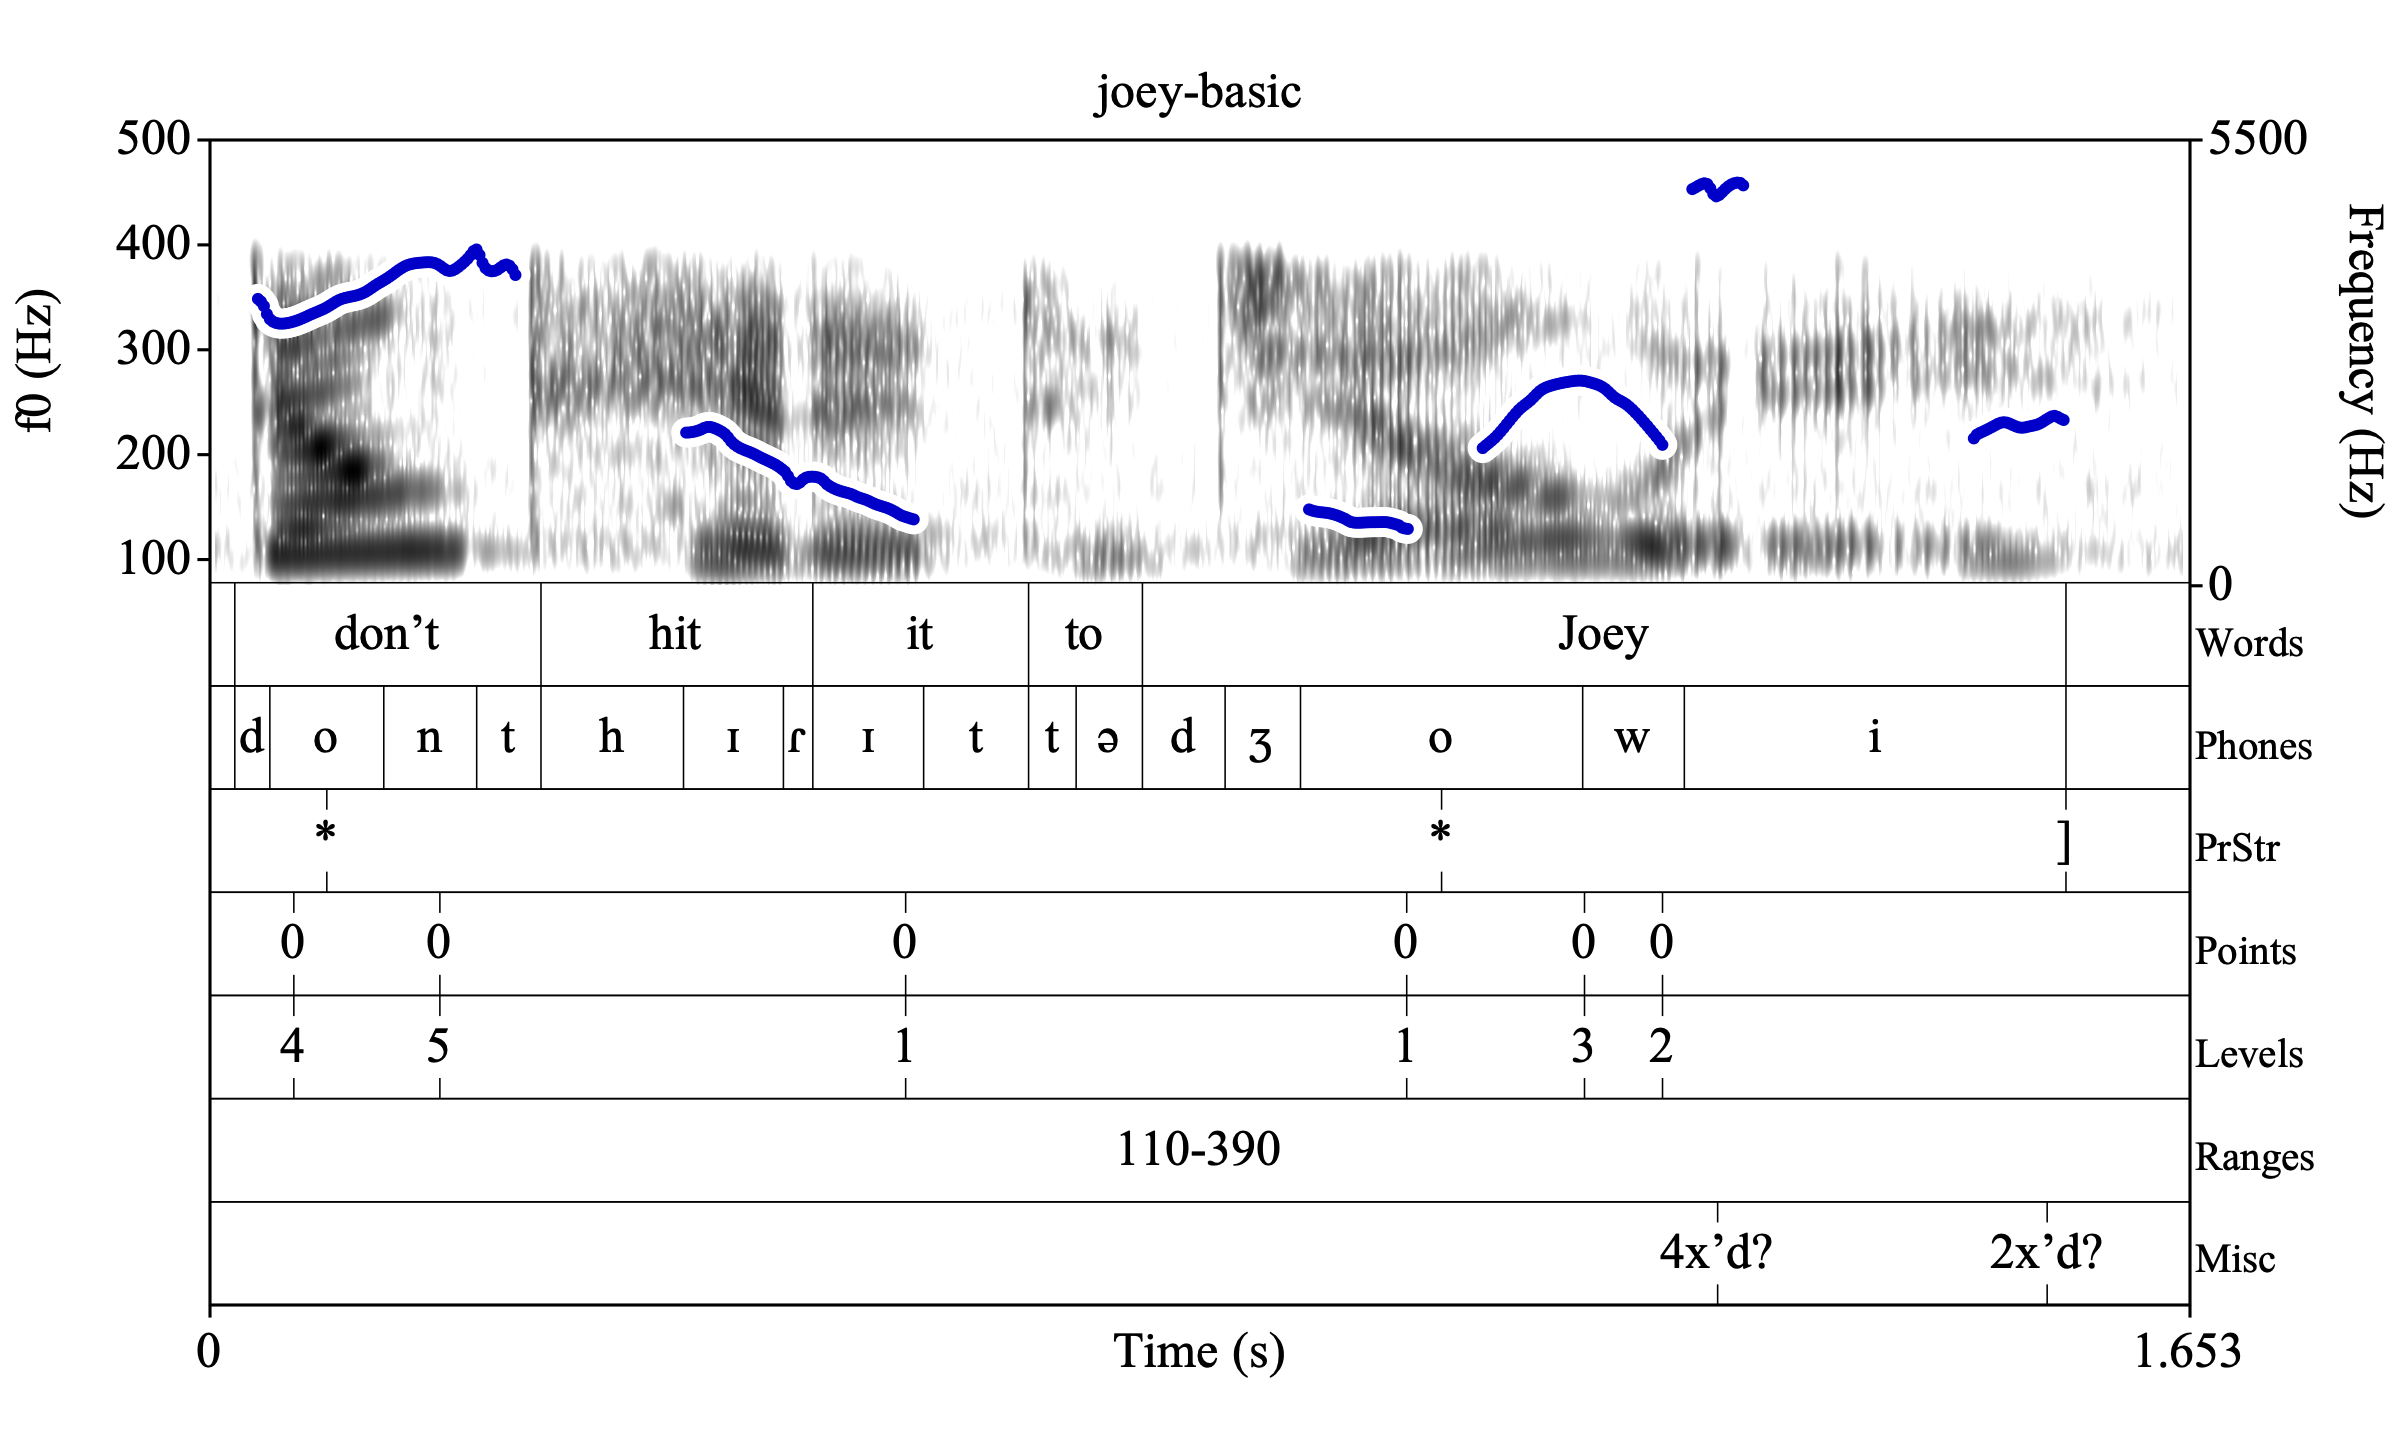
\includegraphics[width=.875\linewidth]{Appendix-joey.png}
\caption{Example of creaky voice phonation disturbing pitch tracking.
\label{fig:joey f0-tracking}
\index{Annotated example, f0 tracking!joey}
}
\end{figure}
Another example of the impact of creaky voice on f0 tracking can be seen in Fig. \ref{fig:no_cigar f0-tracking}. From the beginning of “\langtext{but}” through the [n] of “\langtext{no}”, there is creaky voice during. During that time, there is no pitch tracking (even during the voiced [ʌ] and [n]), and when the f0 tracking returns, it appears to be high and falling onto the [o]; however, this f0 fall is due to the offset of creaky voice, and auditory perception indicates  that the pitch is steadily rising during “but no” (as reflected in Points labels). (Notice also that there are segmental effects from the [s] and [g] of “\langtext{cigar}".)
\begin{figure}[H]
\centering
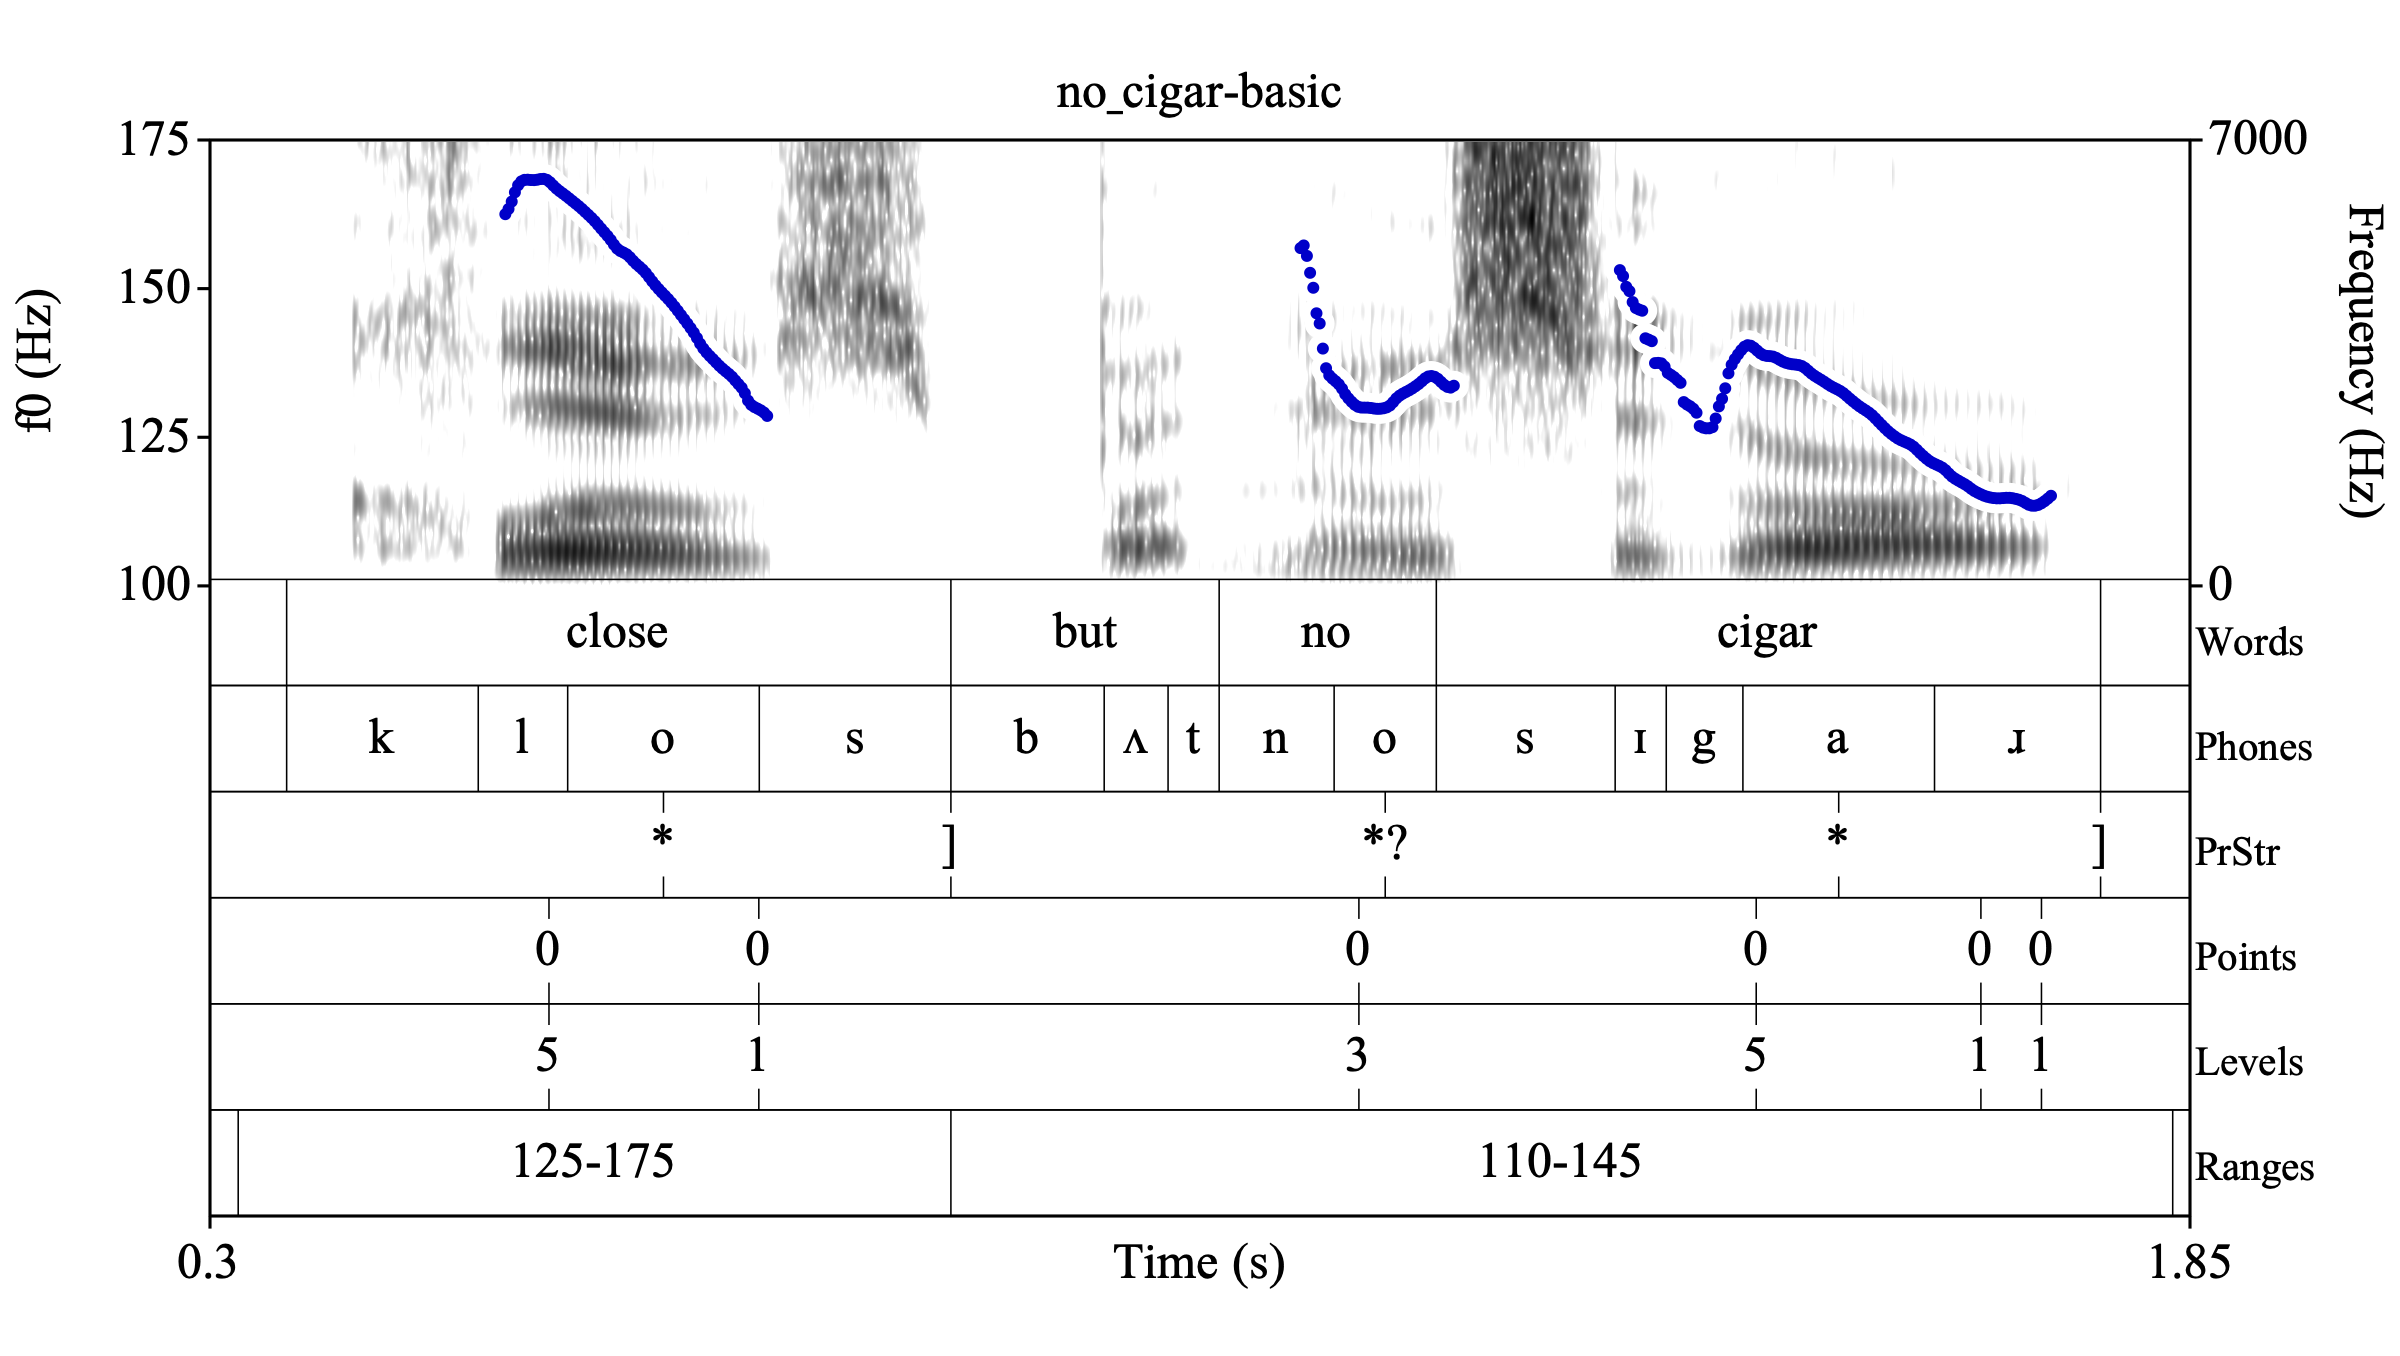
\includegraphics[width=.875\linewidth]{Levels-no_cigar-basic.png}
\caption{Example of creaky voice phonation disturbing pitch tracking.
\label{fig:no_cigar f0-tracking}
\index{Annotated example, f0 tracking!joey}
}
\end{figure}
\subsection{Guiding principles for recognizing and dealing with pitch track disruptions}\label{sec:guiding-principles-for-recognizing-and-dealing-with-pitch-track-disruptions}
\begin{enumerate} \def\labelenumi{\arabic{enumi}.}
\item If the f0 appears to change locally in a way that is surprisingly rapid and not clearly part of a bigger pitch pattern, consider the context in which those bumps, spikes or jumps are occurring. Could they be due to segmental effects or pitch tracking errors? Is the “pitch range” in the “pitch settings”
\item In PoLaR labelling, where possible, put Points labels at places in the signal where you believe that the f0 measured corresponds to the pitch you perceive at that region of the utterance
\item For places where you believe a point or range floor or ceiling occurs during unreliable pitch, estimate what the f0 value should be at that point. (See detailed guidelines in the Advanced Points labelling section.) 
\end{enumerate}
\bibliographystyle{glossa.bst}
\bibliography{ch2.bib}
\end{document}	